\documentclass[        
    a4paper,% Tamanho da folha A4
    12pt,               % Tamanho da fonte 12pt
    sumario=tradicional,
    %chapter=title,     % Todos os capitulos devem ter caixa alta
    %section=TITLE,     % Todas as secoes devem ter caixa alta
    oneside,            % Usada para impressao em apenas uma face do papel
    english,            % Hifenizacoes em ingles
    spanish,            % Hifenizacoes em espanhol
    brazil% Ultimo idioma eh o idioma padrao do documento
]{abntex2/abntex2}

\usepackage[utf8]{inputenc} % UNICODE no arquivo tex
\usepackage[T1]{fontenc}    % UNICODE no arquivo pdf
\usepackage{amsmath}
\usepackage{multicol}
\DeclareMathOperator{\arcsec}{arcsec}
\usepackage{subfigure}
\usepackage[compatibility=false]{caption}

%\usepackage[small,bf]{caption}
\usepackage{graphicx}                               % Inserir figuras
\usepackage{amsfonts, amssymb, amsmath, amsthm, exscale, ifthen}             % Fonte e símbolos matemáticos
\usepackage{booktabs}                               % Comandos para tabelas
\usepackage{verbatim}                               % Texto é interpretado como escrito no documento
\usepackage{multirow, array}                        % Múltiplas linhas e colunas em tabelas
\usepackage{indentfirst}                            % Endenta o primeiro parágrafo de cada seção.
\usepackage{listings}                               % Utilizar codigo fonte no documento
\usepackage{xcolor}
\usepackage{microtype}                              % Para melhorias de justificação?
\usepackage[portuguese,ruled,lined]{algorithm2e}    % Escrever algoritmos
\usepackage{algorithmic}                            % Criar Algoritmos  
\usepackage{float}                                  % Utilizado para criação de floats
\usepackage{amsgen}
\usepackage{lipsum}                                 % Usar a simulação de texto Lorem Ipsum
\usepackage{tocloft}                                % Permite alterar a formatação do Sumário
\usepackage{etoolbox}                               % Usado para alterar a fonte da Section no Sumário
\usepackage[nogroupskip,nonumberlist,acronym]{glossaries}                % Permite fazer o glossario
\usepackage{caption}                                % Altera o comportamento da tag caption
\usepackage[abnt-repeated-author-omit=yes,alf,abnt-emphasize=bf,bibjustif,recuo=0cm,abnt-etal-cite=2,abnt-etal-list=0]{abntex2cite}  % Citações padrão ABNT
%\usepackage[bottom]{footmisc}                      % Mantém as notas de rodapé sempre na mesma posição
\usepackage[bottom=2cm,top=3cm,left=3cm,right=2cm]{geometry}
%\usepackage{lmodern}                               % Usa a fonte Latin Modern
%\usepackage{subfig}                                % Posicionamento de figuras
%\usepackage{scalefnt}                              % Permite redimensionar tamanho da fonte
\usepackage{color, colortbl}                       	% Comandos de cores
%\usepackage{lscape}                                % Permite páginas em modo "paisagem"
%\usepackage{ae, aecompl}                           % Fontes de alta qualidade
%\usepackage{picinpar}                              % Dispor imagens em parágrafos
\usepackage{latexsym}                              	% Símbolos matemáticos
%\usepackage{upgreek}                               % Fonte letras gregas
\usepackage{appendix}                               % Gerar o apendice no final do documento
\usepackage{paracol}                                % Criar paragrafos sem identacao
\usepackage{lib/uecetex2}		                    % Biblioteca com as normas da UECE para trabalhos academicos
\usepackage{pdfpages}                               % Incluir pdf no documento
\usepackage{amsmath}                                % Usar equacoes matematicas
\usepackage{footnote}                               % Permite footnote em tabelas
\usepackage{subfigure}

\usepackage{longtable}

\setlength\extrarowheight{10pt}                     % Definir altura de linhas das tabelas.

% Organiza e gera a lista de abreviaturas, simbolos e glossario
\makeglossaries

% Gera o Indice do documento
\makeindex

\hyphenation{bacharelado universidade computação garanhuns}

\newcommand{\ok}{$\surd$}
\newcommand{\cf}{\emph{Cloud Foundry}~}

% Definição
\newtheorem{defi}{Definição}

\usepackage{calligra}

% Hifenização
\usepackage{hyphenat}
\tolerance=1
\emergencystretch=\maxdimen
\hyphenpenalty=10000
\hbadness=10000
\hyphenchar\font=-1
\sloppy


% Remove as bordas vermelhas e verdes do PDF gerado
% Coloque 'sim' pare remover
\removerbordasdohyperlink{sim} 

% Adiciona a cor Azul a todos os hyperlinks
\cordohyperlink{sim}

\ies{Universidade Federal Rural de Pernambuco}
\iessigla{UFRPE}
\centro{Programa de Pós-Graduação em Informática Aplicada}

\graduacaoem{Ciência da Computação}
\habilitacao{bacharel}

%TODO - Nome do autor
\autor{Gerson Rodrigues Santos}

%TODO - Título do trabalho
\titulo{Modelos Computacionais para a Simulação e Análise da Detecção de Ondas Gravitacionais.}

%TODO - Ano
\data{2020}

%TODO - Local
\local{Recife -- PE}

%TODO - Data da defesa.
\dataaprovacao{19 de 02 de 2020.}

%%%%%%%%%%%%%%%%%%%%%%%%%%%%%%%%%%%%%%%%%%%%%
%%     Informação sobre o Orientador       %%
%%%%%%%%%%%%%%%%%%%%%%%%%%%%%%%%%%%%%%%%%%%%%

%TODO - Nome do orientador
\orientador{Prof. Tiago A. E. Ferreira}
\orientadorcentro{Universidade Federal Rural de Pernambuco}
\orientadories{Departamento de Estatística e Informática}
\orientadorfeminino{nao} % Coloque 'sim' se for do sexo feminino

%%%%%%%%%%%%%%%%%%%%%%%%%%%%%%%%%%%%%%%%%%%%%
%%      Informação sobre o Co-orientador   %%
%%%%%%%%%%%%%%%%%%%%%%%%%%%%%%%%%%%%%%%%%%%%%

% Deixe o nome do coorientador em branco para remover do documento

\coorientador{Prof. Antônio de Pádua Santos}
\coorientadorcentro{Universidade Federal Rural de Pernambuco}
\coorientadories{Departamento de Física}
\coorientadorfeminino{nao} % Coloque 'sim' se for do sexo feminino

%%%%%%%%%%%%%%%%%%%%%%%%%%%%%%%%%%%%%%%%%%%%%
%%      Informação sobre a banca           %%
%%%%%%%%%%%%%%%%%%%%%%%%%%%%%%%%%%%%%%%%%%%%%

% Atenção! Deixe o nome do membro da banca em branco para remover da folha de aprovacão

%TODO - Primeiro membro da banca
\membrodabancadois{WILSON ROSA DE OLIVEIRA JUNIOR}
\membrodabancadoiscentro{Universidade}
\membrodabancadoisies{Departamento}

%TODO - Segundo membro da banca
\membrodabancatres{Membro 3 da banca}
\membrodabancatrescentro{Universidade}
\membrodabancatresies{Departamento}

\membrodabancaquatro{}
\membrodabancaquatrocentro{}
\membrodabancaquatroies{Universidade do Membro da Banca Quatro - SIGLA}
\membrodabancacinco{}
\membrodabancacincocentro{}
\membrodabancacincoies{Universidade do Membro da Banca Cinco - SIGLA}
\membrodabancaseis{}
\membrodabancaseiscentro{}
\membrodabancaseisies{Universidade do Membro da Banca Seis - SIGLA}

\begin{document}

	% Elementos pré-textuais
	
	\imprimircapa
	\imprimirfolhaderosto{}
	
	\imprimirfichacatalografica{elementos-pre-textuais/ficha-catalografica}
	
	\imprimirfolhadeaprovacao{}
	\imprimirdedicatoria{elementos-pre-textuais/dedicatoria}
	\imprimiragradecimentos{elementos-pre-textuais/agradecimentos}
	\imprimirepigrafe{elementos-pre-textuais/epigrafe}
	\imprimirresumo{elementos-pre-textuais/resumo}
    \imprimirabstract{elementos-pre-textuais/abstract}
	\imprimirlistadeilustracoes
	\imprimirlistadetabelas
    \imprimirlistadealgoritmos
	\imprimirlistadesimbolos{elementos-pre-textuais/lista-de-acronimos}   
	\imprimirsumario
	
	%Elementos textuais
	
	\textual
	\chapter{Introdução}
\label{cap:introducao} 

As Ondas Gravitacionais (\textit{Gravitational waves}) (GW) foram uma previsão da teoria da relatividade geral de Einstein em 1915 \cite{albert1920realtivity}. Devido a seus efeitos mensuráveis serem minúsculos, os cientistas levaram vários anos para detectar suas consequências mais convincentes \cite{cervantes2016brief}. Em 2015, essas pequenas ondulações no espaço-tempo foram detectadas pelo avançado Observatório de Ondas Gravitacionais por Interferometria a Laser (\textit{Advanced Laser Interferometer Gravitational Wave Observatory}) (aLIGO) \cite{PhysRevLett.116.131103, 0264-9381-32-7-074001}.

Dez observações de fusão de buracos negros foram feitas até o final de 2019 \cite{Abbott_2019}, as quais permitiram estudos das propriedades populacionais dos buracos negros de massa estelar e permitiram a realização de testes de precisão da relatividade geral \cite{collaboration2018binary}. E esse grande avanço científico, digno do Prêmio Nobel de Física de 2017, deu inicio a uma nova era na astronomia e astrofísica \cite{huerta2017boss}.

Há um investimento muito forte nesta nova areá emergente de pesquisa, com previsão de que, nos próximos anos novos observatórios no Japão e na Índia entrem em operação, formando uma grande rede de detectores em evolução capaz de observar centenas de fontes de ondas gravitacionais todos os anos \cite{PhysRevD.100.063015}.

Concomitantemente, o aparecimento de novas tecnologias na área da computação provocou um aumento significativo nas pesquisas, em especial, de novos algoritmos computacionais em Aprendizado de Máquina (\textit{Machine Learning}), que é uma técnica de Inteligência Artificial (IA) que se vale de um método de análise de dados a partir da construção e automatização de modelos analíticos \cite{bisong2019building}. Esta tecnologia vem sendo frequentemente usada para auxiliar em vários procedimentos nas mais diversas áreas como, por exemplo, a utilização de IA na realização do processamento de imagens de lesões dermatológicas ou exames radiológicos, de ultrassom, de ressonância magnética, de tomografia, dentre outros, a fim de realizar a automação de diagnósticos patológicos, facilitando assim o trabalho dos profissionais, permitindo que os laboratórios mantenham a qualidade ao manipular o elevado número de amostras diárias \cite{lobo2017inteligencia}.

Em destaque a estas pesquisas podem-se citar as Redes Neurais Artificiais (RNA). As RNAs são técnicas computacionais que visam imitar o funcionamento dos neurônios de organismos inteligentes através de modelos matemáticos. Com esses modelos, é possível treinar, testar e validar a RNA e utilizar a rede treinada para simulações, reconhecimento de padrões, previsão, entre outras aplicações \cite{haykin2011neural}.

Sendo uma dessas aplicações a utilização de Redes Neurais Profundas (\textit{Deep Learning}), uma derivação das redes neurais, na realização do processamento de ondas gravitacionais, detectadas pelo aLIGO \cite{shen2017denoising,PhysRevLett.120.141103,krastev2019real,gebhard2019convolutional,mukund2017transient,kim2015application, george2017deep, george2018deep, PhysRevD.100.103025, Lin2019, Luo2020}, a fim de agilizar as observações desses eventos e rapidamente disseminar suas informações aos laboratórios parceiros para maximizar a chance de observações eletromagnéticas.

Apesar desses resultados preliminares promissores no processamento de ondas gravitacionais utilizando \textit{Deep Learning}, \cite{PhysRevD.100.063015} acreditam que o papel preciso que a IA possa desempenhar dentro do escopo mais amplo das pesquisas de coalescências binárias compactas (CBCs) e da astronomia prática de ondas gravitacionais ainda não foi testado em detalhes suficientes.

No entanto, isto apenas motiva a analise cuidadosa sobre o potencial prático do uso da IA para a procura de GWs de CBCs. Ocasionando, uma crescente busca de soluções cada vez mais eficientes que tenha uma identificação confiável e precisa em tempo real, como é o exemplo de vários trabalhos desenvolvidos nos últimos anos com este objetivo.
    
\section{Delimitação do Tema}
\label{sec:delimitacao-do-tema}

A natureza nem sempre pode ser observada em sua plenitude, mas sempre poderá ser simulada computacionalmente desde que existam os apropriados modelos computacionais. Neste sentido, a computação científica e numérica desempenha o papel de ferramenta fundamental da área da ciência da computação para o entendimento da natureza, explicitando fenômenos e dinâmicas muitas vezes não possíveis de serem observados pela limitada capacidade humana de observação.

Capacidade essa que também não pode acompanhar a avalanche de informações produzidas por muitos dos experimentos de astrofísica e astronomia de hoje. Os quais, alguns deles registram terabytes de dados todos os dias e a quantidade de dados produzida a cada dia está apenas aumentando. O \textit{Square Kilometer Array}, um radiotelescópio programado para realizar as primeiras observações científicas em meados de 2020, será capaz de gerar um tráfego de dados maior que a Internet inteira a cada ano \cite{ska-dewdney2009square, scaife2020big, greig2020reionization}.

Por esse motivo, os pesquisadores passaram a depender de tecnologias integradas para serem capazes de lidar com esse grande fluxo de dados e o uso efetivo desses dados tornou possível aprimorar os métodos de pesquisa, transformando a forma de se fazer ciência. E a RNA se insere nesse contexto justamente para auxiliar os pesquisadores nessa missão. Ela nos permite extrair novos \textit{insights} das informações disponíveis para melhorar a busca de anomalias e detectar padrões que humanos nunca poderiam ter visto.

Existe uma grande gama de problemas que podem ser estudados e resolvidos com as RNAs, porém não existe um modelo pronto de rede que se encaixe na resolução de todos os problemas, cada RNA é construída com base no problema que se deseja resolver, o que em muitos casos torna a construção da rede neural um processo complexo que requer tempo e experiência para a construção de uma rede que consiga atingir bons resultados \cite{barros2018avaliaccao}. 

Ao construir uma RNA é necessário configurar os muitos parâmetros que a compõem, que podem variar de problema para problema e influenciar o resultado positivamente ou negativamente, tais como: dados de entrada, quantidade de camadas ocultas, a quantidade de neurônios em cada camada oculta, o bias, funções de ativação, realimentação da rede, taxa de aprendizagem, entre outros parâmetros dependentes do tipo treinamento da RNA. Existem diversos algoritmos de treinamento, cada um com seus prós e contras, que se encaixam nas diversas categorias de problemas, utilizar o algoritmo correto para a categoria de problemas certa, faz com que a rede consiga solucionar o problema desejado e seja confiável.

\section{Problema de Pesquisa}
\label{sec:problema-de-pesquisa}

A busca pela detecção de ondas gravitacionais continua intensa, a análise e o tratamento computacional destas informações encontram-se na crisa da onda da tecnologia computacional para o entendimento de tal processo.

Para que seja possível a detecção de ondas gravitacionais é necessário um grande esforço contínuo dos detectores e das instalações astronômicas, a natureza sensível a tempo dessas análises requer algoritmos que possam detectar e caracterizar esses eventos em tempo real. A técnica de filtragem combinada(\textit{Matched filtering}, na sigla em inglês), que é uma técnica de processamento de sinais, em que, correlaciona um sinal atrasado conhecido, ou forma de onda, com um sinal desconhecido para detectar a presença da forma de onda no sinal desconhecido \cite{turin1960introduction, Schutz_1999}, provou ser bem-sucedida na descoberta de GWs de CBC a partir dos dados dos observatórios de ondas gravitacionais aLIGO e Advanced Virgo (aVIRGO) \cite{gebhard2019convolutional}.

No entanto, o custo computacional das buscas por GWs usando as atuais técnicas de filtragem combinadas, aumenta significativamente quando é necessário a busca por sinais em uma grande quantidade de dados \cite{abbott2018prospects}.

Além disto, os algoritmos de busca de parâmetros que  representam o sistema detectado, algumas vezes são surpreendidos com incertezas o que causa uma diminuição na acurácia do método usado e um aumento significativo no intervalo de confiança dos parâmetros encontrado.

Por outro lado, por mais que os métodos que utilizam \textit{Deep Learning} mostrem que podem realmente ser efetivamente aplicados a esse problema ao tratá-lo como uma tarefa de classificação binária \cite{gebhard2019convolutional}, ainda necessitam do uso da computação de alto desempenho (HPC do inglês, \textit{high performance computing}), limitando as pesquisas a grupos e laboratórios com acesso a super computadores. Além disso, a própria natureza das redes neurais profundas a tornam um processo custoso quanto ao seu preparo e desenvolvimento. No caso das redes neurais profundas o treinamento pode demorar muito tempo e demandar grandes recursos computacionais.

Para aprimorar ainda mais o alcance científico desse campo emergente, há uma necessidade premente de aumentar a confiabilidade e a velocidade dos algoritmos de ondas gravitacionais que permitiram essas descobertas inovadoras.

\section{Objetivos}
\label{sec:objetivos}

A seguir serão apresentados os objetivos geral e específicos que nortearão a condução desta pesquisa.

\subsection{Objetivo Geral}
\label{sec:objetivo-geral}

A presente pesquisa tem como objetivo geral o desenvolvimento de um classificador binário simples capaz de classificar de forma eficiente as reais medidas das ondas gravitacionais disponíveis pelo aLIGO, baseado em um Comitê de Redes Neurais Artificiais e Analise de score.

\subsection{Objetivo Específico}
\label{sec:objetivo-especifico}

Para atingir o objetivo geral foram definidos os seguintes objetivos específicos: 
\begin{itemize}

\item Obter os modelos das ondas gravitacionais descobertas pelo aLIGO, disponíveis no GWOSC \cite{vallisneri2015ligo} e simular computacionalmente as ondas gravitacionais para a criação do conjunto total de dados;
\item Desenvolver arquiteturas de redes neurais que abranja o problema proposto.
\item Ajustar os parâmetros que melhor se ajustem para o treinamento e validação da RNA;
\item Aplicar uma nova abordagem por analise de score aos resultados da rede. 
\item Desenvolver um Comitê de Redes Neurais Artificiais com as arquiteturas propostas para a classificação de sinais de ondas gravitacionais
\item Validar o Comitê desenvolvido com as reais medidas das ondas gravitacionais do aLIGO.

\end{itemize}

\section{Justificativa}
\label{sec:justificativa}


Com base em todas as considerações descritas, precisamos de um novo paradigma para superar as limitações e os desafios computacionais dos algoritmos de detecção de GW existentes, eliminando assim a necessidade do uso de super computadores, e libertando a pesquisa de ondas gravitacionais a qualquer ambiente computacional.

Um candidato ideal para este feito seria a \textit{Machine Learning}, mais especificamente um Comitê de Redes Neurais Artificiais, o qual, hoje é tendência no mercado, que é uma área  altamente escalável que pode aprender diretamente a partir de dados brutos, usando camadas hierárquicas de redes, em combinação com técnicas de otimização baseadas em retro-propagação e gradiente descendente~\cite{barca2005treinamento}. 

A \textit{Machine Learning}, especialmente com o auxílio da computação GPU, que é encontrada na maioria dos hardwares pessoais, alcançou recentemente um imenso sucesso em aplicações comerciais e em Inteligência Artificial \cite{esteva2017dermatologist, moravvcik2017deepstack, van2016wavenet, 10.1007/978-3-319-44188-7_16}, e também tem sido aplicado em astrofísica \cite{shen2017denoising,PhysRevLett.120.141103,krastev2019real,gebhard2019convolutional,mukund2017transient,kim2015application,george2018deep,george2017glitch, george2017deepA}.

É neste contexto que se insere este trabalho, o qual, busca uma solução confiável simples e eficiente na busca por GWs de CBCs nos dados do aLIGO, utilizando Rede Neurais Artificiais.

\section{Organização do trabalho}
\label{sec:organizacao-do-trabalho}

O presente trabalho está organizado em 5 capítulos e um Apêndice, a saber: Introdução, Fundamentação Teórica, Metodologia, Resultados, Conclusão e Apêndice A. 

A seguir, são descritos resumidamente o conteúdo de cada um dos capítulos seguintes.

Na Fundamentação Teórica são apresentados conceitos sobre ondas gravitacionais e redes neurais artificiais. Na seção sobre ondas gravitacionais, é descrito uma breve explicação do que são ondas gravitacionais, suas fontes, tipos de sinais e como gerar formas de ondas com cálculos físicos. Na seção das redes neurais, descreve-se o neurônio artificial, algumas arquiteturas de redes e o processo de aprendizagem utilizado no trabalho (retro-propagação). 

No capítulo Metodologia, são descritas as ferramentas computacionais utilizadas, o tratamento dos dados obtidos do LIGO e o processo de geração de formas de ondas, juntamente com o processo de ajustes de parâmetros e de aprendizagem das redes neurais geradas (MLPs), e por ultimo, o arranjo das MLPs com o comitê de redes neurais.

O capítulo de Resultados apresenta os resultados obtidos com a aplicação dos dados reais do LIGO sobre o comitê de redes neurais treinadas, descreve as arquiteturas de redes neurais desenvolvidas e a que melhor se adequou ao problema de estudo, qual o melhor processo para a realização do treinamento das redes neurais e os critérios que levaram a esta descoberta.

No capítulo Conclusão são apresentados discussões sobre o trabalho como todo, ressaltando alguns detalhes observados nos Resultados, apresenta quais os ganhos e possíveis trabalhos futuros com descobertas já preestabelecidas.

É mostrado no Apêndice A os gráficos de score gerados pelo comitê de redes neurais para cada uma das ondas gravitacionais obtidas do aLIGO utilizadas neste trabalho.
	\chapter{Revisão da Literatura}
\label{chap:revisao-da-literatura}
\section{Ondas Gravitacionais}
\label{sec:ondas-gravitacionais}
\subsection{Introdução}
\label{subsec:ondas-gravitacionais:introducao}

Qualquer objeto com massa exerce uma força de atração sobre outros objetos com massa, conhecida como “gravidade”. De acordo com a teoria da gravidade de Sir Isaac Newton \cite{newton1687philosophiae}, quaisquer dois objetos exercem uma atração gravitacional um sobre o outro de igual valor e sentido oposto, quando uma massa muda de posição, todo o campo gravitacional em todo o universo muda instantaneamente, e as forças gravitacionais resultantes são instantaneamente alteradas de acordo.

Mas a Teoria da Relatividade Geral de Einstein \cite{albert1920realtivity}, afirma que nenhuma informação pode viajar mais rápido que a velocidade da luz, incluindo informações sobre as posições de massa no universo, que são comunicadas através do campo gravitacional. A Relatividade Geral prevê que uma mudança no campo gravitacional viajará pelo universo à velocidade da luz e são exatamente essas mudanças no campo gravitacional que são as ondas gravitacionais.

De forma geral, as ondas gravitacionais podem ser pensadas como as ondas criadas quando jogamos pedras na superfície de um lago. Essas ondas são perturbações na geometria do próprio espaço-tempo emitidas por colisões violentas que acontecem no universo, que se propagam à velocidade da luz, carregando informações sobre suas origens, bem como pistas sobre a natureza da própria gravidade \cite{LSC-VIRGO, abbott2016observation, ramos2018teoria}.

\begin{figure}[ht]
\centering
\includegraphics[width=.9\textwidth]{figuras/binary-wave_tn.jpg}
\caption{A impressão artística de ondas gravitacionais de dois buracos negros em órbita. [Imagem: T. Carnahan (NASA GSFC)]}
\label{fig:space-time}
\end{figure}

Ondas gravitacionais são criadas por massas móveis, da mesma forma que ondas eletromagnéticas são criadas por cargas em movimento. Mas como a gravidade é a mais fraca das quatro forças fundamentais (sendo as outras o eletromagnético, o nuclear fraco e o nuclear forte), as ondas gravitacionais são extremamente pequenas, produzindo um deslocamentos da ordem de \(10^{-18}\) metros, isto é, 1000 vezes menor que o diâmetro de um próton \cite{abbott2016observation}. Ondas dessa força serão produzidas por sistemas muito massivos que passam por grandes acelerações, como dois buracos negros em órbita que estão prestes a se fundir um com o outro. Como sistemas como esses são raros, essas fontes estarão a anos-luz de distância.

\subsection{Fontes e tipos de ondas gravitacionais}
\label{subsec:ondas-gravitacionais:fontes}

Em geral, qualquer aceleração que não seja esfericamente ou cilindricamente simétrica produzirá uma onda gravitacional \cite{abbott2017gw170814}. Considere uma estrela que vai se transformar em uma supernova, esta explosão produzirá ondas gravitacionais se a massa não for ejetada de maneira esférica simétrica, embora o centro de massa possa estar na mesma posição antes e depois da explosão. Outro exemplo é uma estrela em movimento. Uma estrela perfeitamente esférica não produzirá uma onda gravitacional, mas sim uma estrela irregular \cite{abbott2017gw170817}.

Com base nessas diferentes fontes, os cientistas do LIGO definiram quatro categorias de ondas gravitacionais: Ondas Gravitacionais Contínuas, Ondas Gravitacionais de Sistemas Binários, Ondas Gravitacionais Estocásticas e Ondas Gravitacionais de colapso gravitacional. Cada categoria gera um conjunto único de "impressões digitais" ou assinaturas vibracionais características que os interferômetros do LIGO podem detectar e que os pesquisadores podem procurar nos dados do LIGO \cite{Christensen_2018}.

Ondas gravitacionais contínuas são produzidas por sistemas que têm uma frequência razoavelmente constante e bem definida. Exemplos disso são sistemas de estrelas binárias ou de buracos negros orbitando um ao outro ou uma única estrela girando rapidamente em torno de seu eixo com uma grande inchaço ou outras imperfeições na sua forma esférica. Espera-se que estas fontes produzam ondas gravitacionais comparativamente fracas, uma vez que elas evoluem ao longo de períodos de tempo mais longos e são geralmente menos catastróficas do que as fontes que produzem ondas gravitacionais de sistemas binários ou de colapso gravitacional \cite{beheshtipour2020deep}, Figura~\ref{figondacontinua}.

\begin{figure}[ht]
\centering
\includegraphics[width=.9\textwidth]{figuras/continuous_tn.jpg}
\caption{Um sinal de exemplo de uma fonte de onda gravitacional contínua. [Image: A. Stuver / LIGO]}
\label{figondacontinua}
\end{figure}

Ondas gravitacionais de sistemas binários são geradas durante o estágio final de vida de sistemas binários, onde os dois objetos se fundem em um. Esses sistemas são geralmente duas estrelas de nêutrons, dois buracos negros, ou uma estrela de nêutrons e um buraco negro cujas órbitas se degradaram até o ponto em que os dois objetos estão prestes a coalescer. À medida que os objetos giram em torno uma do outro, suas distâncias orbitais diminuem, retirando parte da energia orbital do sistema, enquanto suas velocidades aumentam \cite{Liu_2018}. Isso faz com que a frequência das ondas gravitacionais aumente até o momento da coalescência, Figura~\ref{figondainspiral}.

\begin{figure}[ht]
\centering
\includegraphics[width=.9\textwidth]{figuras/inspiral_tn.jpg}
\caption{Um sinal de exemplo de uma fonte de onda gravitacional de sistemas binários. [Image: A. Stuver / LIGO]}
\label{figondainspiral}
\end{figure}

As ondas gravitacionais de colapso gravitacional vêm de fontes desconhecidas ou imprevistas de curta duração. Há hipóteses de que alguns sistemas, como supernovas ou rajadas de raios gama, podem produzir ondas gravitacionais de colapso gravitacional, mas pouco se sabe sobre os detalhes desses sistemas para antecipar a forma que essas ondas terão \cite{Christensen_2018}, Figura~\ref{figondacolapso}.

\begin{figure}[ht]
\centering
\includegraphics[width=.9\textwidth]{figuras/burst_tn.jpg}
\caption{Um sinal de exemplo de uma fonte de onda gravitacional de colapso. [Image: A. Stuver / LIGO usando dados de C. Ott, D. Burrows e outros]}
\label{figondacolapso}
\end{figure}

Ondas gravitacionais estocásticas são as ondas gravitacionais relíquias da evolução inicial do universo. Assim como radiação cósmica de fundo em micro-ondas(Cosmic Micro-wave Background - CMB), que provavelmente é a luz residual do Big Bang, essas ondas gravitacionais surgem de um grande número de eventos aleatórios e independentes combinados para criar um fundo de ondas gravitacionais cósmicas. Essas pequenas ondas de todas as direções compõem o que é chamado de sinal estocástico, tendo um padrão aleatório que pode ser analisado estatisticamente, mas não previsto com precisão \cite{Christensen_2018}.

Espera-se que o Big Bang seja o principal candidato para a produção dos muitos processos aleatórios necessários para gerar ondas gravitacionais estocásticas e, portanto, podem conter informações sobre a origem e a história do universo \cite{Christensen_2018}, Figura \ref{figondaestocastica}.

\begin{figure}[ht]
\centering
\includegraphics[width=.9\textwidth]{figuras/stochastic_tn.jpg}
\caption{Um sinal de exemplo de uma fonte de onda gravitacional estocástica. [Imagem: A. Stuver / LIGO]}
\label{figondaestocastica}
\end{figure}

\subsection{Equações de ondas Gravitacionais}
\label{subsec:ondas-gravitacionais:equacoes}

Uma maneira de se entender esse fenômeno matematicamente é através do cálculo que produz esse tipo de evento. Segundo a RG de Einstein, esses efeitos gravitacionais são descritos através da métrica $G_{\mu \nu}(x)$, que traz consigo informação acerca da curvatura do espaço-tempo.

Mas a equação de Einstein constitui um conjunto de 10 equações diferenciais parciais não lineares, o que, torna esse cálculo exaustivo e complexo. Uma maneira atrativa de se pensar nas equações de onda gravitacional produzidas por um sistema binário é tratar cada componente do sistema como um partícula. Segundo \cite{rubbo2007hands}, podemos fazer isto com a seguinte equação:

\begin{equation} \label{eqGW1}
\begin{split}
h(t) = \mathcal{A}(t)\cos \Phi(t),
\end{split}
\end{equation}

Na Equação \ref{eqGW1}, o $h(t)$ é a forma de onda gravitacional produzida pelos componentes(partículas) do sistema, também conhecida como deformação da onda gravitacional, $\mathcal{A}(t)$ é a amplitude dependente do tempo e $\Phi (t)$ é a fase da onda gravitacional. Ainda, segundo \cite{rubbo2007hands}, a amplitude $\mathcal{A}(t)$ pode ser expressa em termos dos parâmetros que caracterizam o sistema,

\begin{equation} \label{eqGW2}
\begin{split}
\mathcal{A}(t) = \frac{2(G\mathcal{M})^{5/3}}{c^4 r} \left(\frac{\pi}{P_{gw}(t)}\right)^{2/3} ,
\end{split}
\end{equation}
onde $G$ é a constante gravitacional de Newton, $c$ é a velocidade da luz, $r$ é a distância da luminosidade ao sistema binário e $P_{gw}(t)$ é o período da onda gravitacional. O valor $M \equiv (M_1 M_2)^{3/5}(M_1+M_2)^{-1/5}$ é a massa do \textit{chirp}\footnote{A massa do \textit{chirp} determina como o sistema evolui e o sinal de onda gravitacional emitido varia em amplitude e frequência, e é derivada da relação entre a massa total do sistema e a sua massa reduzida.} e comumente é usada na física das ondas gravitacionais, como uma escala de massa natural.

A fase das ondas gravitacionais, $\Phi (t)$, é análoga à fase para outro fenômeno das ondas, onde representa a localização do ciclo da onda que está colidindo com o detector no tempo $t$ e acompanha a evolução da amplitude da onda em função do tempo. A fase possui unidades de radianos e está relacionada à frequência da onda gravitacional $f_{gw}$ ou alternativamente ao período $P_{gw} = {f_{gw}^{-1}}$ pela integral da equação \ref{eqGW3}, onde, $\Phi_0$ é o valor da fase inicial, $\Phi_0=\Phi(t=0)$.

\begin{equation} \label{eqGW3}
\begin{split}
\Phi(t) = \Phi_0 + 2\pi \int_0^t \! \frac{{dt}^{'}}{P_{gw}(t^{'})}.
\end{split}
\end{equation}

Seguindo o exemplo dado em \cite{rubbo2007hands}, em que, os valores típicos da equação de amplitude de onda dado na Equação \ref{eqGW2}, foram substituídos por valores de um sistema binário de estrela de nêutrons localizado no centro de nossa galáxia, o mesmo afirma que as ondas gravitacionais são extremamente fracas e a amplitude de $\mathcal{A}$ é adimensional, portanto, a radiação gravitacional se manifesta na matéria ao induzir uma tensão. 

Em outros termos, a Equação \ref{eqGW1} proporciona a mudança relativa na distância entre dois pontos no espaço-tempo em função do tempo, tornando possível medir a separação entre duas massas e verificar se essas massas estão gerando uma onda gravitacional.

Como no eletromagnetismo, as ondas gravitacionais têm dois estados de polarização independentes designados por $\boldsymbol{+}$ e $\mathrm{X}$, como mostra a Figura \ref{figpolarization}. A polarização fornece, entre outras coisas, informação sobre a inclinação do plano orbital de um sistema binário em relação ao observador. Para um sistema binário, os dois estados são relacionados por uma mudança de fase de $90°$. Quando a linha de observação é paralela ao plano orbital do sistema, cada uma das componentes aparenta mover-se numa linha reta e neste caso possível, mostrar que a polarização das ondas gravitacionais emitidas será linear. 

\begin{figure}[ht]
\centering
\includegraphics[width=.9\textwidth]{figuras/polarization.png}
\caption{Modos de polarização das ondas gravitacionais $\mathrm{h_{+}}$ e $\mathrm{h_{x}}$ propagando-se na direção $\mathrm{z}$. [Imagem: \cite{centrella2010black}]}
\label{figpolarization}
\end{figure}

Se, pelo contrário, a linha de observação for normal ao plano orbital, o movimento dos componentes será circular e a polarização observada será também circular. Entre estes dois casos limite existe uma gama de valores possível para a inclinação do plano orbital que pode em princípio ser deduzida através da polarização do sinal observado.

Consequentemente, a Equação \ref{eqGW1} captura a forma funcional dos dois estados de polarização. \cite{rubbo2007hands} afirma que ondas gravitacionais transportam energia e momento angular para longe do sistema binário, fazendo com que o período orbital diminua com o tempo, de acordo com

\begin{equation} \label{eqGW4}
\begin{split}
P_{orb}(t) = \left(P_0^{8/3} - \frac{8}{3}kt \right)^{3/8}
\end{split}
\end{equation}
onde $P_0$ é o período orbital no tempo $t = 0$, e $k$ é uma constante de evolução dada por:

\begin{equation} \label{eqGW5}
\begin{split}
k \equiv \frac{96}{5}(2\pi)^{8/3} \left(\frac{G\mathcal{M}}{c^3}\right)^{5/3}
\end{split}
\end{equation}

Como resultado do período orbital decrescente, os dois componentes binários se aproximaram lentamente, até o ponto em que colidem e coalesce em um único objeto remanescente, que ocorre quando $P_{orb}(t) = 0$.

Portanto, com a Equação \ref{eqGW1} é possível criarmos formas de ondas gravitacionais como mostra a Figura \ref{figmetade}. No entanto, é possível notar que a Equação \ref{eqGW1} não produz forma de onda, em que, o tempo é negativo, $P_{orb}(t) < 0$. Sendo assim, as formas de onda geradas por esse modelo não geram onda após a coalescência dos componentes. Devido a esta limitação este método de geração de ondas gravitacionais não será usado nesta pesquisa.

\begin{figure}[ht]
\centering
\includegraphics[width=.9\textwidth]{figuras/metade.png}
\caption{A forma de onda no último segundo antes da coalescência. Com a amplitude e a frequência do sinal aumentando com o tempo [Imagem: \cite{rubbo2007hands}]}
\label{figmetade}
\end{figure}

Esta é uma das maneiras que os astrônomos de ondas gravitacionais tem de extrair informações astrofísicas das formas de onda de sistemas binários observados. Claro que a análise de sinais reais é mais complexa. O principal desafio para a análise de dados reais é identificar o sinal oculto em um fluxo de dados com ruído. A abordagem mais comumente utilizada para esse problema na astronomia de ondas gravitacionais é usar a filtragem por coincidência. Se um sinal estiver presente em um fluxo de dados barulhento, o modelo fornecerá uma maneira de subtrair o ruído e deixar uma forma de onda limpa. Esta atividade assume que um modelo de sinal foi selecionado. Os astrônomos estimam os valores dos parâmetros astrofísicos que descrevem uma fonte de ondas gravitacionais a partir de formas de onda limpas \cite{rubbo2007hands}. 

\section{Redes Neurais Artificiais}
\label{sec:redes-neurais-artificiais}

\subsection{Introdução às Redes Neurais Artificiais}
\label{subsec:redes-neurais-artificiais:introducao}

Qualquer que seja o organismo multicelular, independente da sua complexidade e organização, possui algum tipo de sistema nervoso que é responsável por alimentar o organismo através de entradas sensoriais sobre informações do ambiente em que o organismo vive. As informações coletadas são processadas e comparadas com experiências passadas e posteriormente são transformadas em ações apropriadas para a situação ou absorvidas em forma de conhecimento \cite{haykin1994neural}.

Para o organismo complexo, humano, o neurônio biológico é basicamente o dispositivo computacional elementar do sistema nervoso que possui muitas entradas e uma saída. As entradas ocorrem através das conexões sinápticas, que conectam a árvore dendrítica aos axônios de outras células nervosas. Os sinais que chegam por estes axônios são pulsos elétricos conhecidos como impulsos nervosos ou potenciais de ação, constituindo a informação que o neurônio processará de alguma forma para produzir como saída um impulso nervoso no seu axônio \cite{kovacs1996redes}. 

O cérebro humano possui uma capacidade incrível de absorção de conhecimento e é considerado o processador mais fascinante que existente, podendo desempenhar funções como percepção, intuição, inferência, reconhecimento de padrões, controle motor, entre outros. Ele possui cerca de $10^{11}$ de neurônios e cada neurônio pode receber de 1.000 a 10.000 contatos sinápticos em seu corpo e dendritos, que são responsáveis por todas as funções e movimentos do nosso organismo. Os neurônios estão conectados uns aos outros através de sinapses, e juntos formam uma grande rede, denominada Rede Neural, que proporciona uma fabulosa capacidade de processamento e armazenamento de informação \cite{kovacs1996redes}, Figura~\ref{figneuronios}. 

\begin{figure}[ht]
\centering
\includegraphics[width=1\textwidth]{figuras/axons.jpg}
\caption{Rede neural humana: o melhor processador de informações existente. [Imagem: \href{ https://neurogestion.wordpress.com}{ https://neurogestion.wordpress.com}]}
\label{figneuronios}
\end{figure}

\subsection{Redes Neurais Artificiais}
\label{subsec:redes-neurais-artificiais:rna}

Há algumas décadas, surgiu a ideia de modelar, computacionalmente, as conexões neurais do cérebro humano, buscando reproduzir as características do neurônio biológico. Neste contexto, as redes neurais artificiais foram desenvolvidas, tomando-se como base as redes de neurônios cerebrais e sinapses biológicas do cérebro humano.

Uma rede neural é um sistema paralelo, distribuído, constituído pela interconexão de unidades básicas de processamento, denominadas neurônios artificiais, que têm a propensão natural para armazenar conhecimento experimental e torná-lo disponível para uso \cite{haykin2011neural}. Todo conhecimento adquirido pela rede se da através de um algoritmo de aprendizagem, cuja função é modificar os pesos de conexões entre os neurônios da rede, conhecidos como pesos sinápticos, de forma ordenada a fim de alcançar o mapeamento desejado.

\subsection{Neurônio Artificial}
\label{subsec:redes-neurais-artificiais:neuronio-artificial}

A menor unidade básica de processamento de uma rede neural artificial é o neurônio, que recebe um sinal de entrada e produz um sinal de saída. O modelo de neurônio mais simples, comumente usado, e que engloba as principais características de uma rede neural biológica, paralelismo e alta conectividade, é o perceptron, representado na Figura~\ref{figperceptron}, que é composto por: m entradas (\(x_1, \ldots ,x_m\)), m pesos sinápticos (\(w_1, \ldots , w_m\)), uma variável de deslocamento linear \(b\) (do inglês: bias) e uma saída \(y\), descrito por:

\begin{equation} \label{eqRNA6}
\begin{split}
y = \theta(\sum_{i=1}^{m} x_i w_i + b)
\end{split}
\end{equation}

\begin{figure}[ht]
\centering
\includegraphics[width=.5\textwidth]{figuras/perceptron.png}
\caption{Modelo do neurônio artificial perceptron. [Imagem: \href{ http://computacaointeligente.com.br}{ http://computacaointeligente.com.br}]}
\label{figperceptron}
\end{figure}

A função \(\theta\) é conhecida como função de ativação ou função de transferência. Dentre as funções de ativação mais utilizadas estão a sigmoide e a tangente hiperbólica, definidas pelas equações abaixo, respectivamente \cite{articlefunclogtan}:

\begin{equation} \label{eq2}
\begin{split}
\theta(u) & = \frac{1}{1+ e^{-au}}\\
\theta(u) & = \frac{e^u - e^{-u}}{e^u + e^{-u}}
\end{split}
\end{equation}

\subsection{Arquitetura de uma RNA}
\label{subsec:redes-neurais-artificiais:arquitetura}

A arquitetura de uma RNA está relacionada com a maneira pela qual os seus neurônios estão organizados. De acordo com \cite{furtado2019redes}, as arquiteturas das RNAs são subdivididas em 3 classes: Rede Neural Feedforward de 1 camada, Rede Neural Feedforward Multicamadas e Redes Recorrentes ou Realimentadas. Além disso, a rede também é dividida em três tipos de camadas: a de entrada, a escondida e a de saída. 


As camadas podem ser classificadas em camadas de entrada, onde os padrões são apresentados à rede; camadas ocultas, onde é feita a maior parte do processamento; e a camada de saída, onde a conclusão do processamento é apresentada \cite{furtado2019redes}. Normalmente uma rede neural possui uma camada de entrada, uma camada de saída e \(k\) camadas ocultas, no qual \(k\) é definido empiricamente e varia de acordo com o problema.

Redes neurais do tipo Feedforward são redes de múltiplas camadas, ou seja, elas tem \(k\) camadas ocultas, no qual, a informação propaga-se da entrada para a saída, no caso, os sinais provenientes dos neurônios de uma camada só podem estimular os neurônios da camada seguinte. Quando a rede possuir todos os nós de uma camada comunicando-se com todos os nós da camada posterior, ela é dita totalmente conectada. Caso alguma das conexões sinápticas não esteja ligada com a camada subsequente, a rede é dita parcialmente conectada \cite{furtado2019redes}. A Figura \ref{figredeFeedforwardMulticamada} representa uma rede Feedforward multicamada de uma camada oculta totalmente conectada, ou seja, $k=1$.

% \begin{figure}[h]
% \centering
% \includegraphics[width=.75\textwidth]{figuras/multicamadas.png}
% \caption{Exemplo de rede neural artificial do tipo Feedforward multicamadas. [Imagem: \cite{furtado2019redes}]}
% \label{figredeFeedforwardMulticamada}
% \end{figure}

\begin{figure}[h]
\centering
\includegraphics[width=.75\textwidth]{figuras/multicamadas.png}
\caption{Exemplo de rede neural artificial do tipo Feedforward multicamadas. [Imagem: \cite{furtado2019redes}]}
\label{figredeFeedforwardMulticamada}
\end{figure}

\subsection{Algoritmo de Treinamento}
\label{subsec:redes-neurais-artificiais:algoritmo}

A arquitetura da rede define, dentre outros parâmetros, a que tipo de treinamento a rede será submetida, capacitando-a a resolver o problema. No processo de treinamento a rede ‘aprende’ através de exemplos que relacionam as entradas e saídas do problema a ser solucionado. Essa abordagem é conhecida como aprendizado supervisionado. Dentre os algoritmos conhecidos, para solucionar esse tipo de problema, o mais utilizado é o backpropagation \cite{rumelhart1986learning}. A ideia do algoritmo é estimar os valores dos pesos e bias minimizando o erro entre a entrada e a saída desejada. O erro \(E\) cometido pela rede é calculado por:

\begin{equation} \label{eq3}
\begin{split}
E = \frac{1}{2} \sum_{i=1}^{p} \sum_{j=1}^{n} (d_{j}^{i} - y_{j}^{i})^2
\end{split}
\end{equation}
no qual, \(p\) é o número exemplos a ser utilizados no treinamento, n é o número de saídas da rede e, finalmente, \(d\) e \(y\) são as saídas desejadas e obtidas, respectivamente, para a entrada em questão.

Se o erro \(E\) encontrado for retropropagado (termo que foi derivado do nome do algoritmo backpropagation) pela rede, isto é, se o erro for propagado a partir da camada de saída até a camada de entrada, ela tentará estabelecer o quanto cada sinapse contribuiu para o erro, e este será usado para ajustá-las. A regra de atualização de cada peso sináptico da rede é calculado pela seguinte equação:

\begin{equation} \label{eqRNA4}
\begin{split}
W = W + \Delta W \therefore \Delta W = - \alpha\frac{\partial E}{\partial W}
\end{split}
\end{equation}

onde, \(\alpha\) é conhecido como taxa de aprendizado, que, resumidamente, indica o ‘tamanho do passo’ do gradiente rumo a minimização. O sinal negativo indica a busca por uma alteração no peso que reduza \(E\), sendo assim, quanto menor o erro, melhor a rede estará mapeando o problema.
	\chapter{Metodologia}
\label{chap:metodologia}

\section{Obtenção e Processamento dos Dados}
\label{sec:obtencao-processamento-dados}

Tanto para o processo de treinamento quanto para o processo de teste de uma RNA, o primeiro passo a ser dado é a obtenção das amostras experimentais para o treinamento supervisionado e teste das RNAs. Algoritmos de aprendizado máquinas supervisionadas são muito mais eficazes quando treinados com conjuntos de dados muito grandes.

Em 1 de dezembro de 2018, o aLIGO Scientific Collaboration e o Virgo Collaboration anunciaram o GWTC-1 \cite{Abbott_2019}, catálogo de GW observadas pelo aLIGO e Virgo durante a primeira e a segunda execução de observações, contendo os resultados completos de suas pesquisas por GW, que conta com onze detecções de GW provenientes dez de sistemas binários de buracos negros e um sistemas binário de estrelas de nêutrons.

O primeiro passo dado nesta pesquisa foi a coleta dos dados das GWs, as quais estão disponíveis no catálogo GWTC-1 através do Gravitational Wave Open Science Center (GWOSC)\footnote{\href{https://www.gw-openscience.org/about/}{ttps://www.gw-openscience.org/about/}}~\cite{vallisneri2015ligo}. Como as fusões de buracos negros dominam o número de detecções de GW, este trabalho focou exclusivamente neste tipo de detecção.

Após a obtenção dos dados, foram analisados e selecionados nove das dez amostras de GW de fusão de buracos negros, sendo elas: GW150914, GW151012, GW151226, GW170104, GW170608, GW170729, GW170809, GW170814, GW170823. As quais foram processadas com a ajuda da ferramenta PyCBC\footnote{\href{https://pycbc.org/}{https://pycbc.org/}}~\cite{alex_nitz_2019_2801307}, que é um pacote de software escrito em Python\footnote{\href{https://www.python.org/}{https://www.python.org/}}, usado para explorar e analisar as fontes astrofísicas de GW, e capaz de detectar binários compactos coalescentes e medir seus parâmetros astrofísicos. O PyCBC contém diversos módulos para processamento de sinais e um deles é capaz de gerar formas de GW. A partir desse módulo foi gerado uma forma de GW equivalente ao formato real das GW capturados pelos detectores de GW (Hanford-H1 e Livingston-L1 Interferômetros) para cada uma das amostras selecionadas.

Devido aos detectores terem uma alta sensibilidade, ruídos de origens instrumentais, ambientais e provenientes de atividades humanas sempre o atingem, poluindo os sinais e dificultando as detecções. Durante todo o processo os dados oriundos do aLIGO foram limpos e filtrados e também ignoradas as falhas, os blips e outras fontes de ruído de detectores transientes que dificultam a analise e processamento das GW.

As formas de GW são geradas como uma série temporal, usando uma das aproximações de forma de onda disponíveis pelo PyCBC. Os parâmetros principais foram as massas do sistema binário (dadas em massas solares), o tempo entre as amostras (em segundos), a frequência inicial das GW (Hz) e o nome do aproximante que gostaríamos de gerar. Está disponível uma variedade de aproximações que incluem diferentes efeitos físicos. A precisão numérica depende da resolução, enquanto a precisão da extrapolação pode ser avaliada pela comparação de diferentes ordens de extrapolação. Pedidos mais altos tendem a produzir melhores resultados na fase inspiral, mas pior na fase do ringdown \cite{scharpf2017simulation}. 

Desta forma optou-se por buscar aproximadores com níveis mais elevados de precisão que tivessem o melhor resultado para ambas as fases das simulações, devido a resultados mais atualizados e mais precisos. Para esta pesquisa foi usado o aproximante IMRPhenomD, pois atende altos níveis de precisão graças a uma combinação de métodos analíticos \textit{post-Newtonian} (PN) e \textit{effective-one-body} (EOB) para descrever a inspiração, e a calibração de modelos fenomenológicos de fusão-ringdown para simulações de relatividade numérica (NR)~\cite{khan2015frequencydomain}. Ele modela a forma de GW nas fases de inspiração, fusão e ringdown dos buracos negros e inclui a capacidade de cada buraco negro girar na mesma direção que a órbita (rotação alinhada), atingindo bons resultados em ambas as fases de inspiral e ringdown. Além de poderem ser geradas rapidamente e para uma ampla gama de valores de parâmetros.

O PyCBC foi usado no projeto descrito nesta tese tanto para geração de banco de modelos quanto todo o processo de filtragem correspondente dos dados brutos advindos do aLIGO. Usamos o PyCBC para geração simples de GW no domínio da frequência com massas e tempo de amostras iguais as dos sistemas binários descritos no catalogo GWTC-1 com uma frequência inicial de 20Hz. Portanto, foram gerados dezoito GW equivalentes as GW detectadas pelo aLIGO, nove para cada detector aLIGO (Hanford-H1 e Livingston-L1).

A escolha e adequação dos dados utilizados para treinar e testar uma RNA é de fundamental importância. É necessário que se disponha de dados em quantidade e qualidade suficientes. Caso a quantidade de dados seja pequena, a rede não conseguirá criar um modelo suficientemente representativo para se ter um desempenho satisfatório quando aplicado em situações reais após o seu desenvolvimento, o que é chamado de sobre-ajuste (overfitting) dos dados. Além disto, os dados devem englobar todos os aspectos do problema em questão, a fim de que o modelo criado seja genérico. 

Como o objetivo é treinar uma RNA que forneça um diagnóstico classificativo entre GW e Ruído, que apresente um bom desempenho, extraímos um intervalo de 0.1 segundos de cada forma de onda com pico centralizado, deslocando a localização de pico de cada sinal aleatoriamente dentro de um intervalo de 0 a 0.05 segundos para a direita, a uma taxa de amostragem de 4096Hz. Este processo foi repetido 600 vezes para cada uma das formas de onda geradas, criando assim 10800 modelos de GW, a Figura~\ref{fig:gw150914-offset} ilustra algumas das ondas geradas.

\begin{figure}[ht]
    \centerline{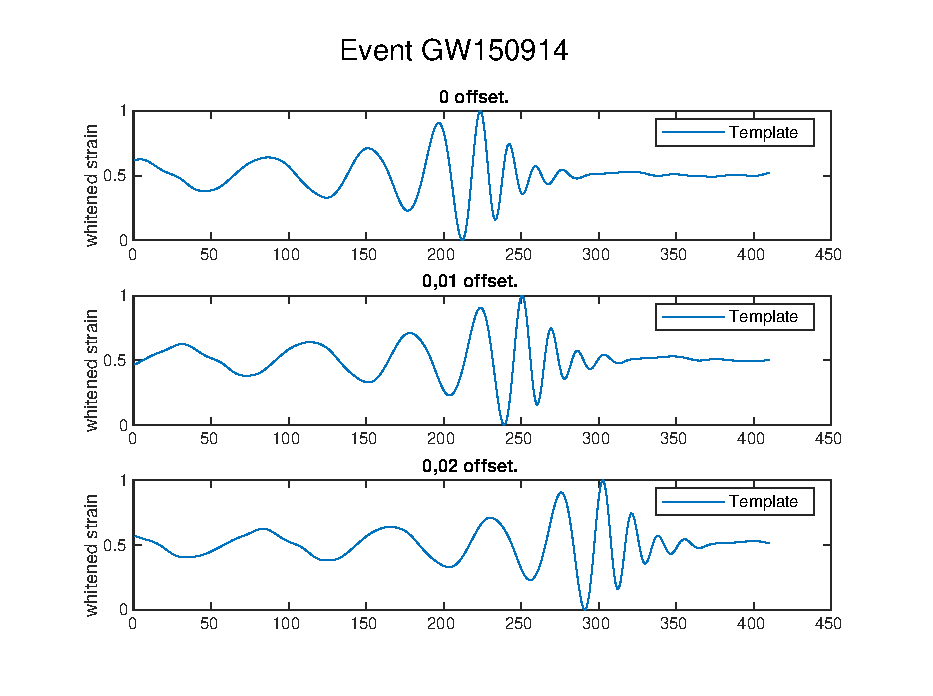
\includegraphics[width=1\textwidth]{figuras/GW150914.eps}}
    \caption{Alguns modelos de GW com deslocamento}
    \label{fig:gw150914-offset}
\end{figure}

Os modelos de machine learning são construídos para minimizar erros. Desde que a probabilidade pertence a classe com maior número de observação, o algoritmo estará enviesado em classificar as novas observações. Afim de evitar o enviesamento por causa do desbalanceamento dos dados, foi criado também a mesma quantidade de amostras de ruído com espectro equivalente a densidade espectral de potência (DEP ou PSD em inglês) do ruido do aLIGO~\cite{T1800044}. No final da construção dos dados, juntamos os dois bancos de dados (ruídos e ondas), totalizando o conjunto de dados de treinamento, teste e validação com um total de 21600 amostras com duas classes: Ondas e Ruídos.

É esperado que uma RNA, após a fase de treinamento, seja capaz de produzir respostas corretas a estímulos externos, mesmo que estes não sejam exatamente iguais aos estímulos utilizados no seu treinamento. Para o conjunto de dados de novos estímulos, foram necessários 2.0 segundos de observação a uma taxa amostral de 4096Hz de cada um das nove GW selecionadas anteriormente, filtradas com a onda centralizada, na qual eles foram separados em várias janelas de 0.1 segundos (410 pontos) com passos de uma unidade e a mesma taxa de frequência amostral, gerando assim aproximadamente ~7780 janelas de dados. Esses dados foram gerados para os dois detectores aLIGO (Hanford-H1 e Livingston-L1) separadamente, totalizando aproximadamente ~140000 de dados.

Alguns algoritmos têm dificuldade em entender variáveis que têm mais do que uma categoria. Pelo fato dos dados apresentarem duas classes categóricas (onda e ruído) o algoritmo de Machine Learning que empregamos nesta pesquisa não produz bons resultados com esses dados categóricos. Diante dessa limitação foi preciso converter as variáveis categóricas para valores numéricos. Buscando melhorar o processamento dos dados foi aplicado uma técnica de pré-processamento de dados chamada one-hot encoding. 

O one-hot encoding é usada em Machine Learning como um método para quantificar dados categóricos e melhorar significativamente os resultados \cite{sarkar2017practical}. Em resumo, esse método produz um vetor com comprimento igual ao número de categorias no conjunto de dados. Neste caso, as classes onda e ruído são transformadas em vetores como: $[1,0]$ e $[0,1]$ respectivamente, que indicam a saída correspondente desejada da RNA para cada uma das classes do conjunto de dados.

Com essa imensa quantidade de dados seria difícil manter tudo sobre estruturas de arquivos simples separados por vírgulas (CSV do inglês comma-separated-values), pois além de consumir muito espaço físico o processo de leitura desses arquivos se tornaria demasiadamente longo. Para resolver este problema, todos os conjuntos de dados foram salvos em HDF (Hierarchical Data Format), que é uma biblioteca de software e formato de dados de alto desempenho (HDF4, HDF5) projetados para armazenar e organizar grandes quantidades de dados para facilitar a leitura dessa grande massa de dados~\cite{hdf}. Por usar árvores B para indexar os dados, o HDF funciona bem para dados de séries temporais. A maior parte dos dados entra em matrizes simples que podem ser acessadas muito mais rapidamente do que as linhas de um banco de dados SQL. 

O HDF foi desenvolvido para processamento e armazenamento de E/S rápidos de alto desempenho com um rico conjunto de recursos de desempenho integrados que permitem otimizações de tempo de acesso e espaço de armazenamento~\cite{hdf}. Esta biblioteca foi amplamente adotada em vários setores e é o padrão de fato na comunidade científica e de pesquisa, uma vez que a maioria das ferramentas que usa Machine Learning suportam esse tipo de arquivo.

\section{Arquitetura da Rede Neural}
\label{sec:arquitetura-rna}

Definir a arquitetura de uma RNA é muito importante devido ao fato de que seu arranjo depende do problema a ser tratado. Ademais, a arquitetura da rede está diretamente relacionada ao algoritmo de aprendizagem usado para treinamento. De acordo com o teorema da aproximação universal, aplicado às redes MLP, uma única camada escondida de neurônios é suficiente para realizar uma aproximação de qualquer função contínua para um dado conjunto de treinamento representado pelo conjunto de entradas e a saídas-alvo \cite{cybenko1989approximation, haykin2007redes}.

Com base nesta premissa, foi desenvolvida uma arquitetura de RNA simples para otimizar e acelerar o processo de treinamento e detecção de GWs. Foi gasto um tempo significativo pesquisando por tentativa e erro uma ótima arquitetura de RNA e otimizando hiperparâmetros. Após sucessivas simulações para determinação do número de entradas das redes neurais, foi estabelecido que a rede neural teria 410 entradas. Sendo assim, cada janela de dados das GW seria apresentados à rede, ou seja, o classificador será aplicado ao fluxo de dados contínuo usando janelas deslizantes de 0,1 segundo de largura com uma diferença de 200 microssegundos.

Diversas estruturas de RNA do tipo MLP com diferentes quantidades de neurônios na camada oculta e diferentes funções de ativação foram testadas visando obter a melhor e mais otimizada estrutura MLP a ser empregada nesta dissertação para a detecção de GWs. Decidir o número de neurônios na camada oculta é um aspecto complexo e um fator que afeta o desempenho das redes treinadas. Segundo \cite{OKOH201619}, a prática mais plausível é treinar várias redes que variam o número de neurônios da camada oculta e, em seguida, selecionar a melhor delas usando um índice de desempenho.

No entanto, foi possível aprimorar ainda mais a discriminação da RNA graças a implementação do \textit{one-hot encoding}, que é um processo pelo qual variáveis categóricas são convertidas em um formato binário que pode ser fornecido aos algoritmos de RNA para fazer um trabalho melhor na classificação \cite{buckman2018thermometer}. Com essa técnica foi possível definir duas categorias quantizadas representadas pelos valores binários de 0 e 1, consequentemente a RNA acompanhou a quantidade de saída desejada e foi colocado duas saídas na última camada da RNA, as saídas A e B. 

Agora, por exemplo, se o estimulo de entrada da rede fosse da classe ``Onda'', as saídas da RNA desejadas seriam A = 1 e B = 0 [1,0] e se o estimulo de entrada fosse da classe ``Ruído'', as saídas da RNA desejadas seriam A = 0 e B = 1 [0,1]. Com essas duas saídas, é possível definir um score como:

\begin{equation}
score = \frac{a-b}{2}+0.5
\label{eq:score}
\end{equation}

Dessa forma, a saída da RNA desejada para a classe Onda terá uma pontuação que tenderá a 1 ($score \rightarrow 1$), e a saída da RNA desejada para a classe Ruído terá uma pontuação que tenderá a 0 ($score \rightarrow 0$). 

Durante o processo de encontrar a melhor estrutura e parâmetros para a rede, o modelo foi avaliado através de uma análise de distribuição dos resultados, do erro quadrático médio (MSE) e do cálculo da estatística de Kolmogorov-Smirnov (KS). Graças ao score desenvolvido na Equação \ref{eq:score}, foi possível construir uma distribuição de pontuação para cada classe, e a capacidade de discriminação da RNA pode ser medida com o uso da distância KS. Essa distância KS é a distância máxima entre duas funções de Distribuição Empírica Acumulada (ECD do inglês \textit{Empirical cumulative distribution}), que quando normalizadas são um valor na faixa [0,1]. O KS é descrito pela teoria estatística não paramétrica e é utilizada para testar se as distribuições de dois grupos são iguais~\cite{daniel2000applied}. 

O teste de KS tem sido utilizado para avaliar o desempenho de classificadores binários avaliando a diferença entre as distribuições dos maus e bons clientes \cite{karcher2009redes} e distribuição do cliente mais propensos a quitar suas dividas ou não \cite{forti2018tecnicas}  por exemplo, neste caso, quanto maior for a estatística de KS, maior será a separação entre os clientes adimplentes e inadimplentes como também entre cliente quitados e não quitados respectivamente. 

Em outras palavras, para esta pesquisa ele avalia o quão bem o modelo consegue distinguir os classificados como Onda dos classificados como Ruído. Sendo assim, o KS se comporta como uma medida de avaliação de performance, quanto maior for o resultado do KS (indicação de maior diferença entre as distribuições), melhor está a acurácia do modelo, pois a separação das classes é maior. 

A estatística de Kolmogorov–Smirnov pode ser descrita por: 
\begin{equation}
KS = Max|F1(x)−F2(x)|
\label{eq:kolmogorov}
\end{equation}
onde $Max$ é a maior distância entre as distribuições de $F1$ e $F2$, em que, $F1$ é a distribuição acumulada do score dos classificados como Ondas e $F2$ é a distribuição acumulada do score dos classificados como Ruído.

É mostrado na Figura~\ref{fig:ANN_Distribution_a} uma ilustração pictórica da distribuição empírica do score gerado para o problema de classificação binária, onde a classe $X$ tem uma distribuição do score centrada em torno de $0$ e a classe $Y$ tem uma distribuição do score em torno de $1$. É mostrado na Figura~\ref{fig:ANN_Distribution_b} a distância KS entre essas duas distribuições.

\begin{figure}[H]
\centering
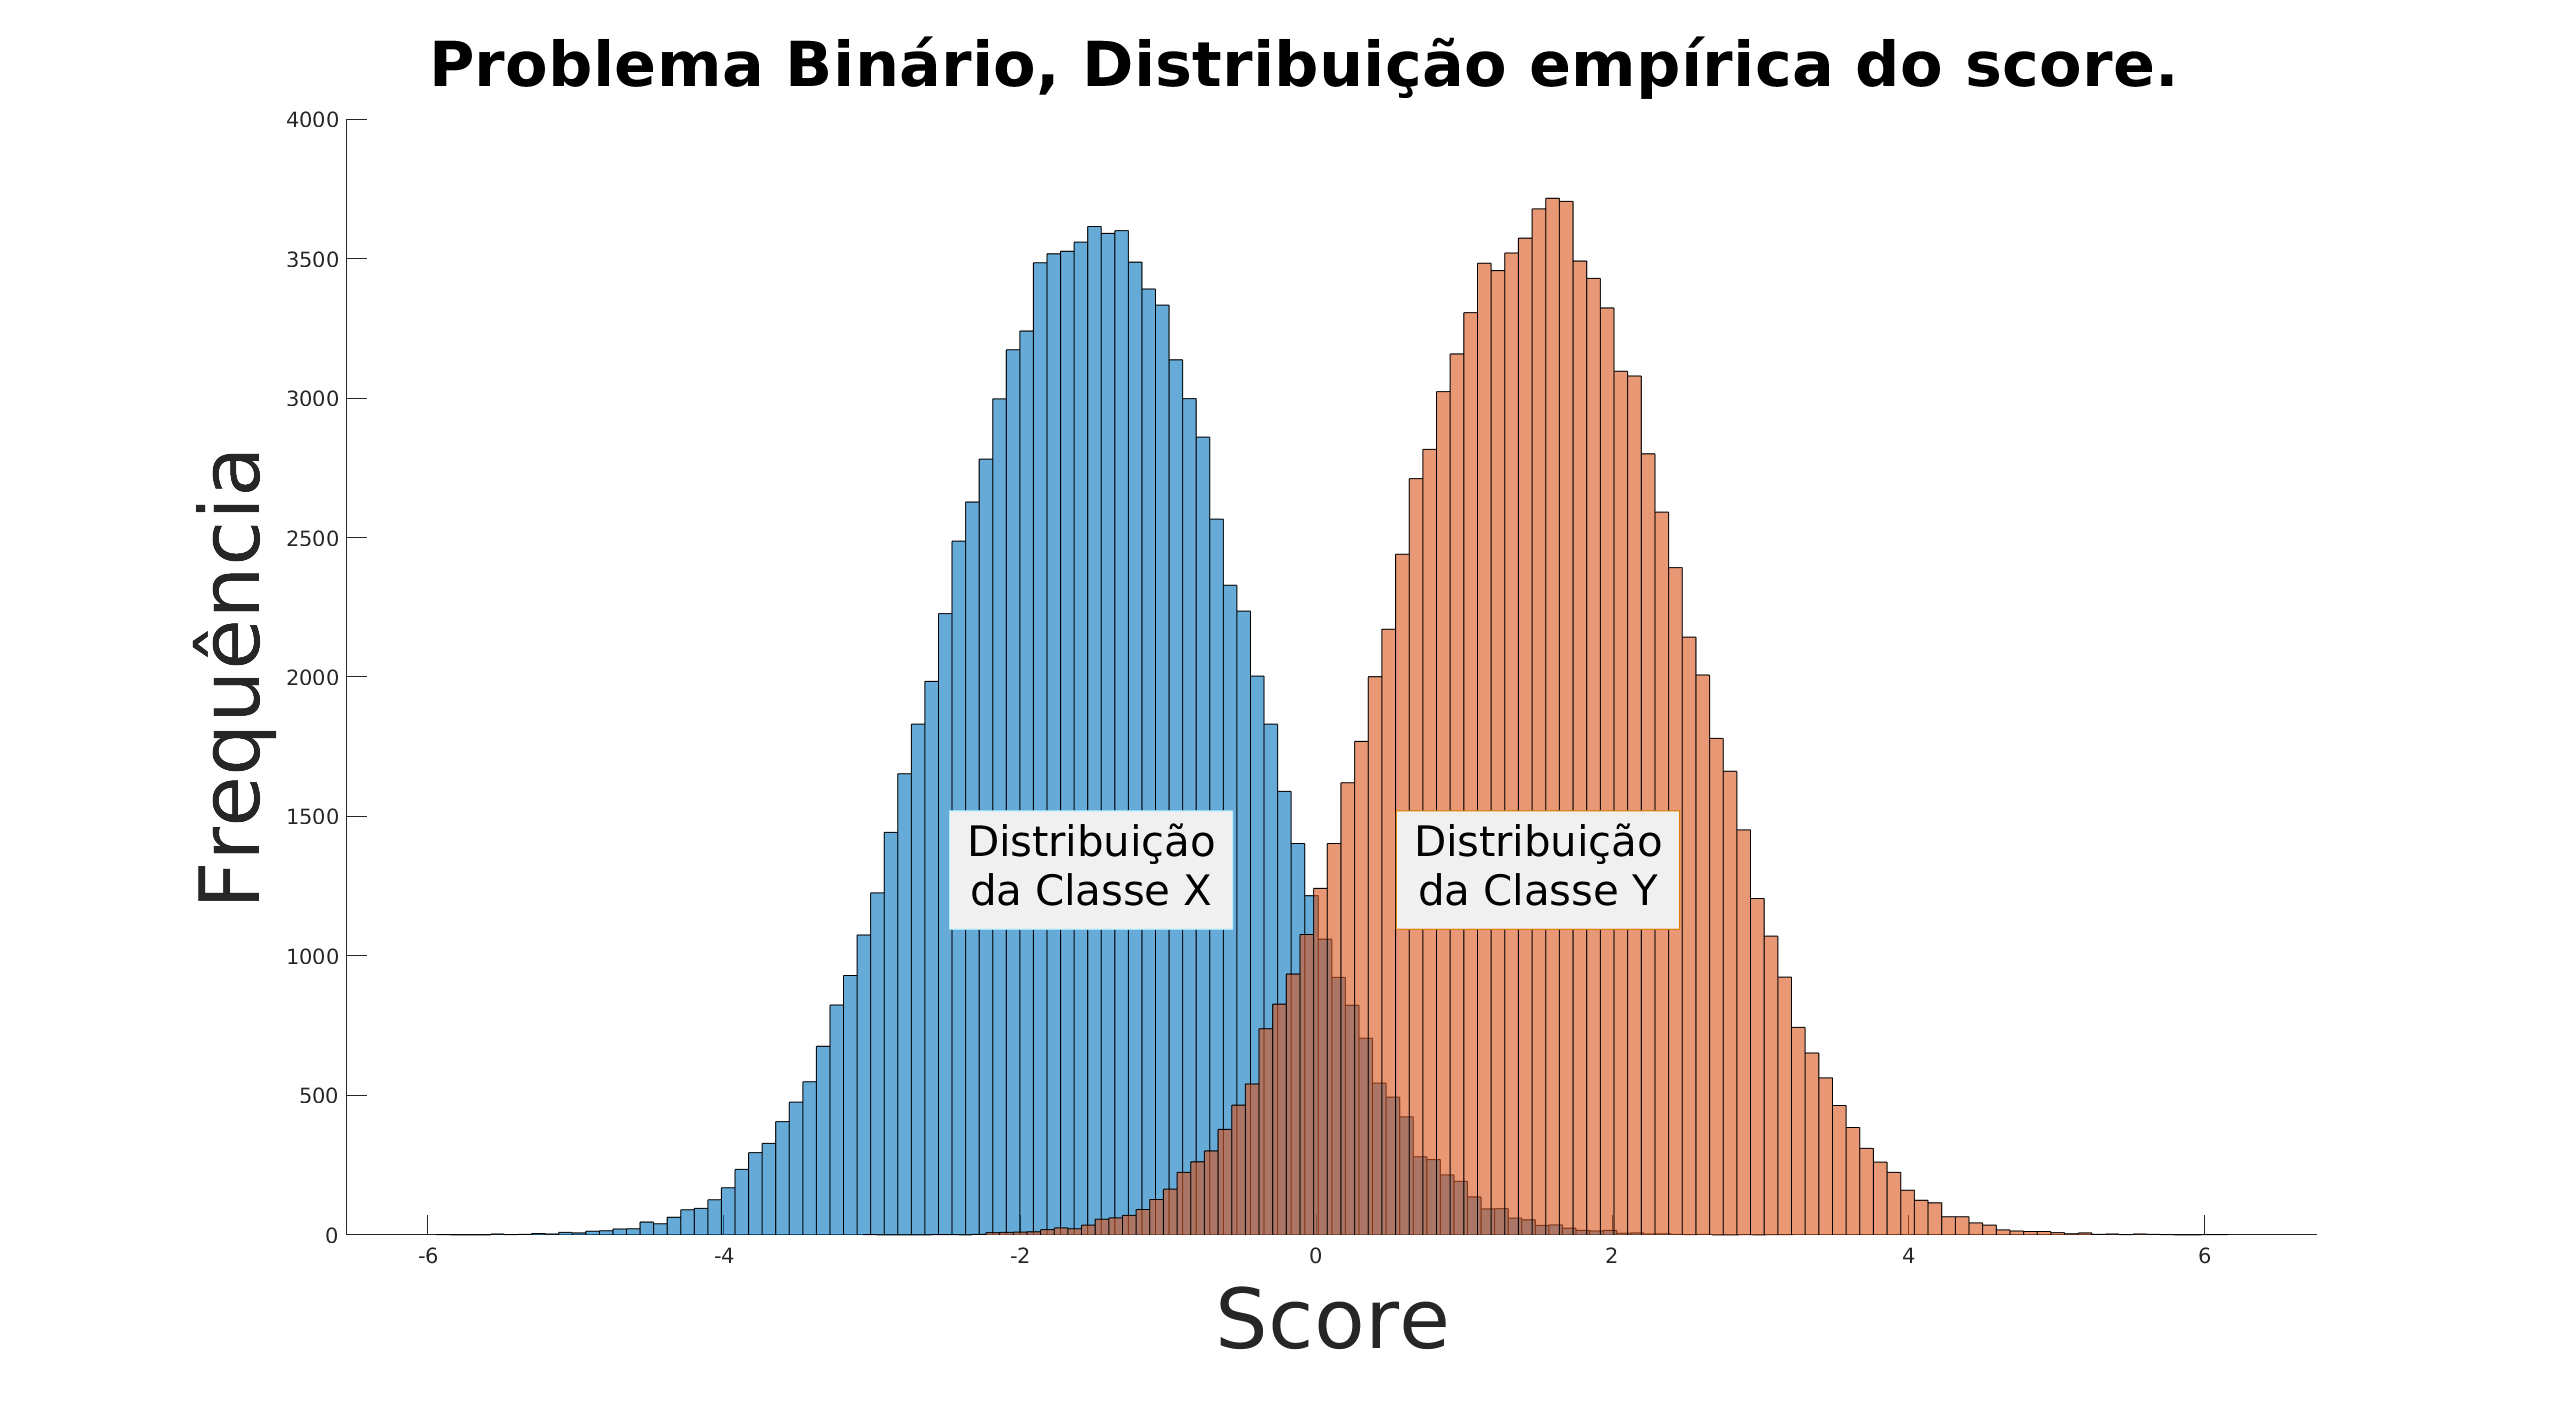
\includegraphics[width=1\textwidth]{figuras/hitograma_distribuicao_empirica_score.eps}
\caption{Resposta pictórica do score da RNA para um problema de classificação binária - Distribuição empírica do score.}
\label{fig:ANN_Distribution_a}
\end{figure}

\begin{figure}[H]
\centering
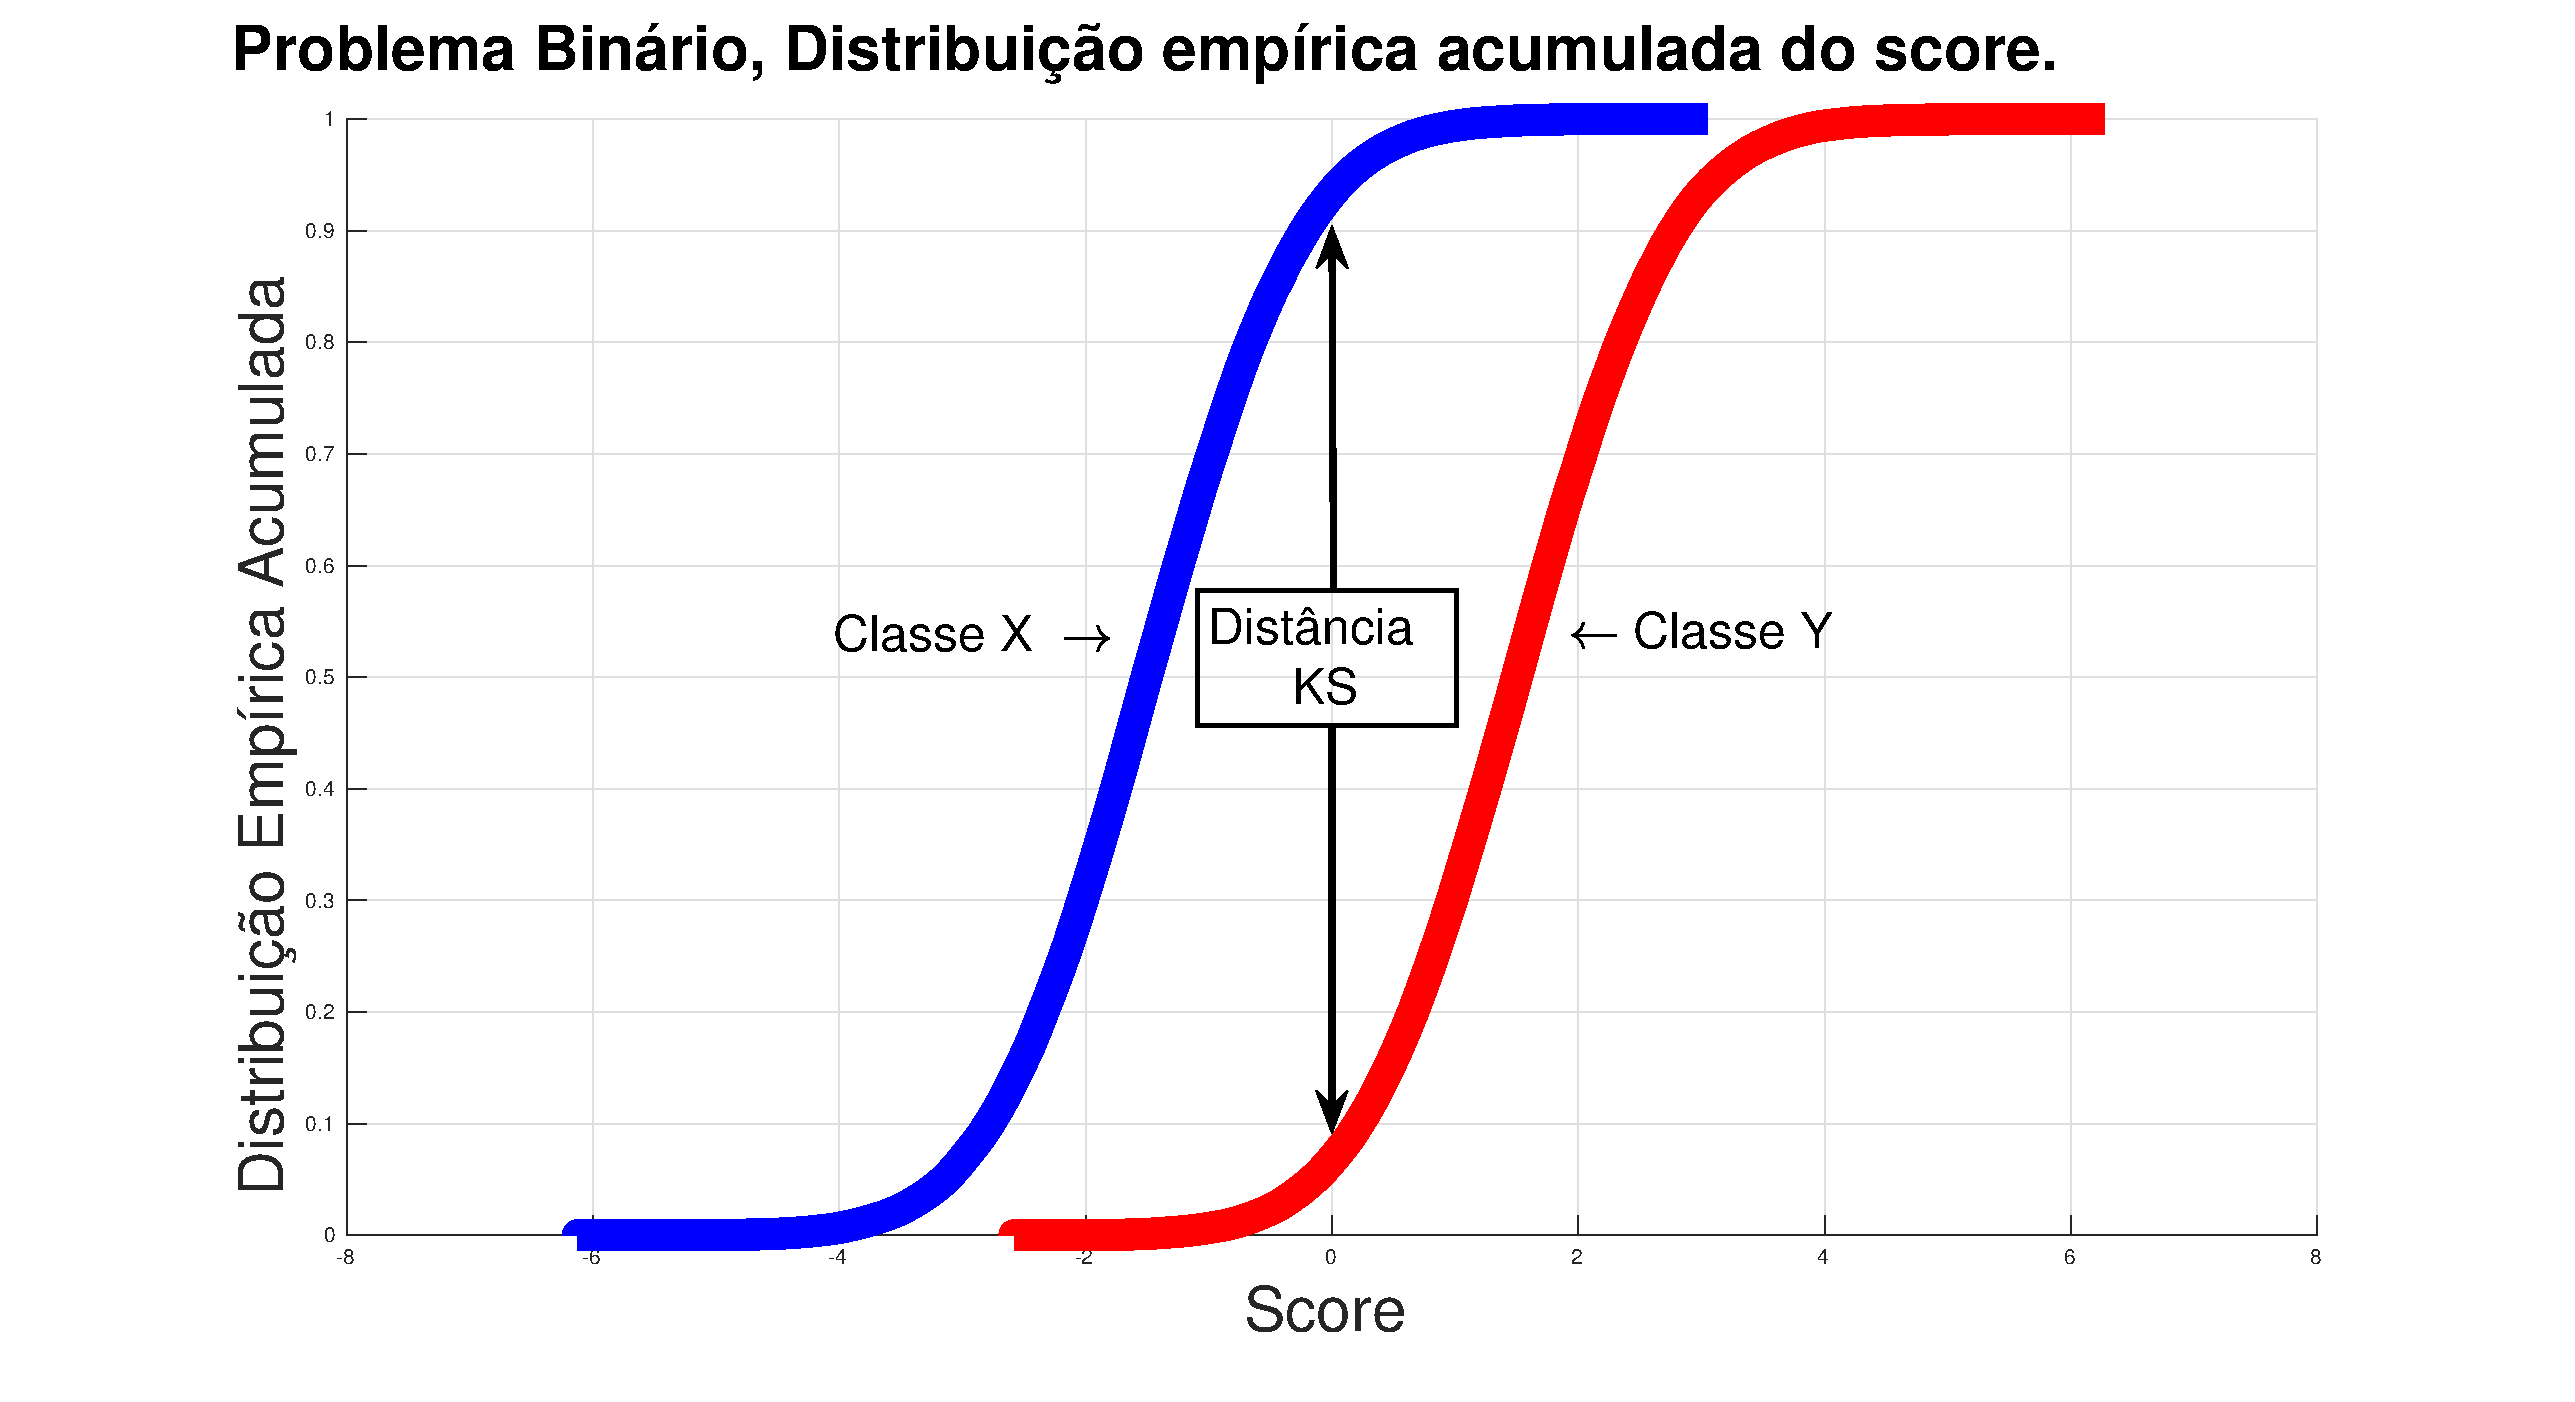
\includegraphics[width=1\textwidth]{figuras/distribuicao_empirica_acumulada_score.eps}
\caption{Resposta pictórica do score da RNA para um problema de classificação binária --- Distribuição empírica acumulada do score.}
\label{fig:ANN_Distribution_b}
\end{figure}

\section{Treinamento da Rede}
\label{sec:treino-rna}

O principal objetivo do processo de aprendizagem de uma RNA é fazer com que um conjunto de entradas produza um conjunto de saídas desejadas ou, no mínimo, um conjunto de saídas aceitável, ao serem aplicadas em uma RNA~\cite{haykin2007redes}.

Para uma RNA, o conceito de treinamento se diferencia do conceito de aprendizado. O aprendizado está associado a uma tarefa que a rede está executando em função do treinamento e da sua modelagem. Já o treinamento é o processo de ensinar a RNA~\cite{furtado2019redes}.

Pode-se dizer que o treinamento da rede neural é o ponto mais critico que determina o desfecho da rede, pois, neste procedimento, a rede é submetida ao aprendizado, onde alguns fatores dos parâmetros de treinamento são relevantes, como: o algoritmo de treinamento, o número máximo de iterações, a taxa de aprendizagem, a função de ativação e muitos outros.

A seleção dos parâmetros de treinamento de uma RNA pode ser um processo complexo, pois pequenas diferenças nestes parâmetros podem levar a grandes diferenças tanto no tempo de treinamento como na generalização obtida.

Nesta pesquisa foram testados diversos algoritmos de aprendizagem, tanto de primeira ordem como de segunda ordem, como RProP, Gradiente Conjugado, Quase-Newton e Levenberg–Marquardt. Contudo, o algoritmo de Backpropagation com taxa de aprendizado adaptativa encontrou os melhores resultados, embora não tenha sido o mais rápido computacionalmente. Para sua utilização, alguns parâmetros inerentes do algoritmo precisaram ser definidos, como: taxa de aprendizagem $\eta$ entre $0.5$ e $0.9$, exceto nos casos de taxa adaptativa, O numero de épocas foi definido com $100000$ épocas.

As funções de ativação são um elemento de extremamente importante das RNAs. Elas basicamente decidem se um neurônio deve ser ativado ou não. Ou seja, se a informação que o neurônio está recebendo é relevante e deve ser propagada ou não~\cite{DeepLearningBook}. Para que se encontrasse a função de ativação que melhor se adequasse as redes desenvolvidas nesta pesquisa, foram usadas somente três funções de ativação, são elas: Linear, Sigmoide e Tangente Hiperbólica.

Uma das dificuldades do processo de treinamento de uma RNA consiste em encontrar o melhor ponto de parada do treinamento, pois o erro de treinamento começa com um valor muito alto, decai rapidamente, e continua diminuindo lentamente, tendendo a atingir um mínimo local na superfície de erro~\cite{haykin2007redes}. Para isto, existem vários métodos para a determinação do momento em que o treinamento de uma RNA deve ser encerrado. Uma boa determinação deste momento é fundamental para um bom treinamento e consequentemente uma boa generalização. Portanto, o treinamento é interrompido quando a rede apresenta uma boa capacidade de generalização e quando a taxa de erro é pequena, menor que um erro aceitável. É necessário encontrar um ponto ótimo de parada com o menor erro possível e capacidade de generalização máxima~\cite{barros2018avaliaccao}.

Neste sentido, o critério de parada no processo de treinamento foi o número máximo de iterações de $100000$ épocas, taxa de erro médio por época de $1e^{-15}$ e sua capacidade de generalização com $100$ validações. Desta forma, o treinamento é encerrado quando qualquer um dos critérios é atendido.

Em relação aos pesos sinápticos, eles foram inicializados com números randômicos, mantendo o cuidado de não serem grandes suficientes para saturarem os neurônios, nem pequenos a ponto de atrasarem o aprendizado.

Para o conjunto de dados, normalmente são separados em dois conjuntos: conjunto de treinamento, que é usado para treinar a rede e conjunto de teste, que é utilizado para verificar a performance da rede sob condições reais de utilização. 

Afim de evitar o problema de overfitting, foi feita um subdivisão do conjunto de treinamento, criando um conjunto de validação, usado para verificar a eficiência da rede quanto a sua capacidade de generalização durante o processo de treinamento, o que se justifica o seu uso como critério de parada do treinamento da rede.

O conjunto de total de dados contém exatos 21600 amostras de dados, separados em duas classes igualmente. Desses dados, 70\% são para treinamento, 15\% para validação e 15\% para teste. O conjunto de dados reais para execução contém aproximadamente ~140.000 padrões de entrada, que são usados para a resolução final da rede executando situações reais com a rede treinada.

Depois de determinar estes conjuntos, eles foram colocados em ordem aleatória para prevenção de tendências associadas à ordem de apresentação dos dados. Além disso, todos os valores de entrada foram normalizados no intervalo [0,1].

\section{Construção do Comitê}
\label{sec:comite}

A grande disponibilidade de recursos computacionais, possibilitou a criação de múltiplas propostas de soluções, as quais foram descartadas como testes e ajustes dos parâmetros para a busca do melhor modelo (rede). Entretanto, visto que, em certo ponto da pesquisa as RNAs descartadas apresentavam um desempenho parecido e com resultados consistentes, foi possível implementar um comitê de redes neurais.

De acordo com \cite{haykin2011neural}, a combinação do conhecimento adquirido pelas RNAs para chegar a uma solução global é supostamente superior àquela obtida por qualquer RNA única. Sendo assim, várias RNAs com a melhor configuração foram treinadas e dentre elas foram selecionadas 500 modelos com o melhor desempenho que formaram a máquina de comitê de redes neurais.

A máquina do comitê desenvolvida na Figura~\ref{fig:comite} mostra um número k, em que k = 500 RNAs treinadas individualmente de maneira independente que compartilham uma entrada comum e cuja saída individual é combinada para produzir uma saída geral. As saídas dessas redes são colocadas em um módulo de combinação que executa a função de calcular a média das saídas combinadas de todas as RNAs do comitê e apresentar o resultado do comitê de RNA.

\begin{figure}[H]
\centering
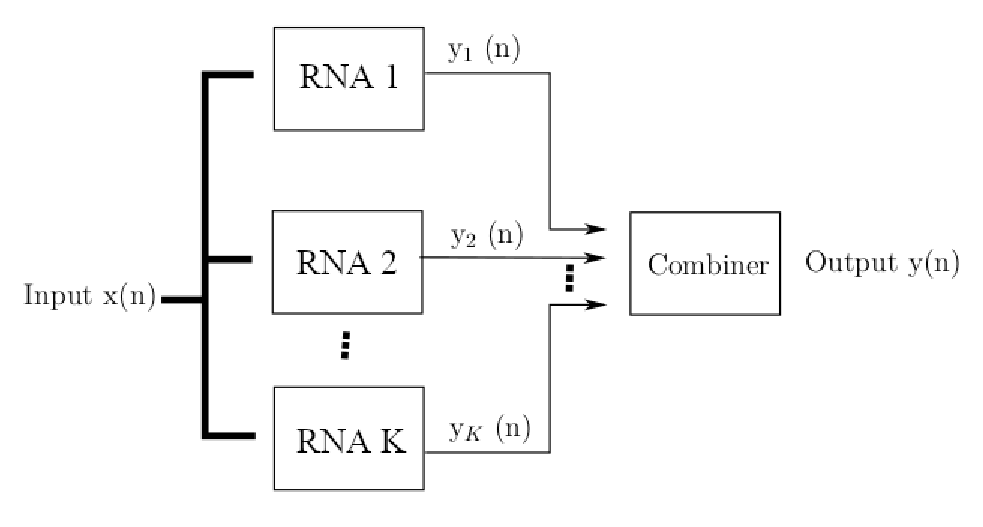
\includegraphics[width=1\textwidth]{figuras/comite.eps}
\caption{Diagrama de blocos de uma máquina de comitê.}
\label{fig:comite}
\end{figure}

Para implementação, execução e teste das RNAs, o software Matlab® R2018b\footnote{\href{ https://www.mathworks.com/products/matlab.html} {https://www.mathworks.com/products/matlab.html}} foi escolhido. Por possuir uma interface gráfica de treinamento de redes neurais, esse aplicativo suporta os mais diversos tipos de algoritmos de treinamento de redes neurais, permitindo que se possa executar uma extensa árvore de testes na tentativa de definir o modelo neural mais adequado, além de seu amplo uso pela comunidade científica.
	\input{elementos-textuais/4resultados}
	\chapter{Conclusão}
\label{chap:conclusao}

Desde a confirmação e descoberta das ondas gravitacionais, muito se falou sobre este assunto, consequentemente muitos estudos voltados a esta área vieram a tona. Mesmo assim, poucos estudos foram feitos mesclando o uso de Machine Learning com as ondas gravitacionais. Diante disto, esta pesquisa se caracteriza como uma grande contribuição nesta areá de pesquisa que aos poucos esta atraindo mais visibilidade. 

Nesta pesquisa foi empregado um comitê de redes neurais com hiperparâmetros rigorosamente ajustados e produzido uma saída em score que retorna uma estatística de classificação equivalente à uma função de pertinência inferida de que os dados contêm um sinal de onda gravitacional, mostrando que o método empregado neste trabalho pode, em princípio, ser usado para pesquisar diretamente sinais GWs nos dados em tempo real e agilizar as observações e rapidamente disseminar suas informações a outros laboratórios  maximizando a chance de outras observações eletromagnéticas. Além disso, foi mostrado nesta pesquisa que com os resultados do comité, o score, é possível extrair informações dos sistemas geradores das ondas gravitacionais, como por exemplo o tempo de ringdown e a reverberação pós fusão dos objetos compactos.

É importante destacar também, que devido a simplicidade da arquitetura das redes neurais desenvolvidas, o método desenvolvido nesta pesquisa é capaz de ser reproduzido em ambientes computacionais mais simples. Além disso, a escalabilidade intrínseca desta metodologia pode superar e abranger o espaço de parâmetros de fusão de buracos negros e ser aplicado a outros tipos de fusão, como sinais de fusão binárias de estrelas de nêutrons e fusão de estrelas de nêutrons com buracos negros. 

Essas capacidades podem permitir pesquisas rápidas e automatizadas de GW em qualquer ambiente, cobrindo milhões ou bilhões de modelos em toda a gama de espaço de parâmetros. Portanto, essa abordagem tem aptidão para aumenta a profundidade e a velocidade do algoritmo desenvolvido, permitindo pesquisas online em tempo real após ser treinado com bancos de modelos de milhões ou bilhões de formas de onda.

\chapter{Trabalhos Futuros}

Os resultados apresentados nesta pesquisa fornecem um forte incentivo para estender a metodologia para a possibilidade de estimativa de parâmetros assim como em~\cite{PhysRevD.97.044039,GEORGE201864}. Futuramente, será investido mais esforço no ajuste de hiperparâmetros e inclusão de novas formas de ondas que abrangem diversos parâmetros de fusões, ao ponto de superar a sensibilidade das pesquisas de Deep Learning e matched-filtering. Ademais, será pesquisado a estimação de parâmetros juntamente com a detecção de sinais nos dados do LIGO, tornando a detecção rápida com a estimativa de parâmetros igualmente rápida, fundamental para a astronomia de ondas gravitacionais.

Essas considerações fornecem motivação suficiente para desenvolver e implantar novas abordagens nesta área de pesquisa afim de produzir um \textit{pipeline} de detecção de sinais de GWs único, simples e computacionalmente eficiente que unifica a detecção em tempo real de GW e a estimativa de parâmetros, em que, qualquer um posso usar e desenvolver novas pesquisas, fazendo deste um método de pesquisa competitivo.

Por tanto, esta nova abordagem tem potencial para penetre a comunidade científica e sirva como um passo fundamental para permitir observações em tempo real de sinais GW, fornecendo alertas imediatos para acompanhamento após eventos de GW. Considera-se que esta nova metodologia para processar sinais em dados ruidosos seja útil em muitas outras áreas, tornando essa metodologia muito promissora para vários campos de pesquisa. Fazendo deste trabalho o alicerce para integralizar diversos setores de especialização para permitir e acelerar descobertas científicas.

No geral, esta pesquisa tem capacidade para se tornar uma ferramenta útil de pesquisa para a analise de GW, mas há um esforço substancial de pesquisa e desenvolvimento para alcançar isso.
	
	%Elementos pós-textuais	
	
	\bibliography{elementos-pos-textuais/referencias}
	\imprimirglossario	
	\imprimirapendices
		% Adicione aqui os apendices do seu trabalho
		\chapter{GRÁFICOS DOS SCORES GERADOS PELO COMITÊ DE REDES NEURAIS}

\section{Score da onda gravitacional GW151012}
\begin{figure*}[ht]
     \subfigure[Score gerado para o laboratório H]{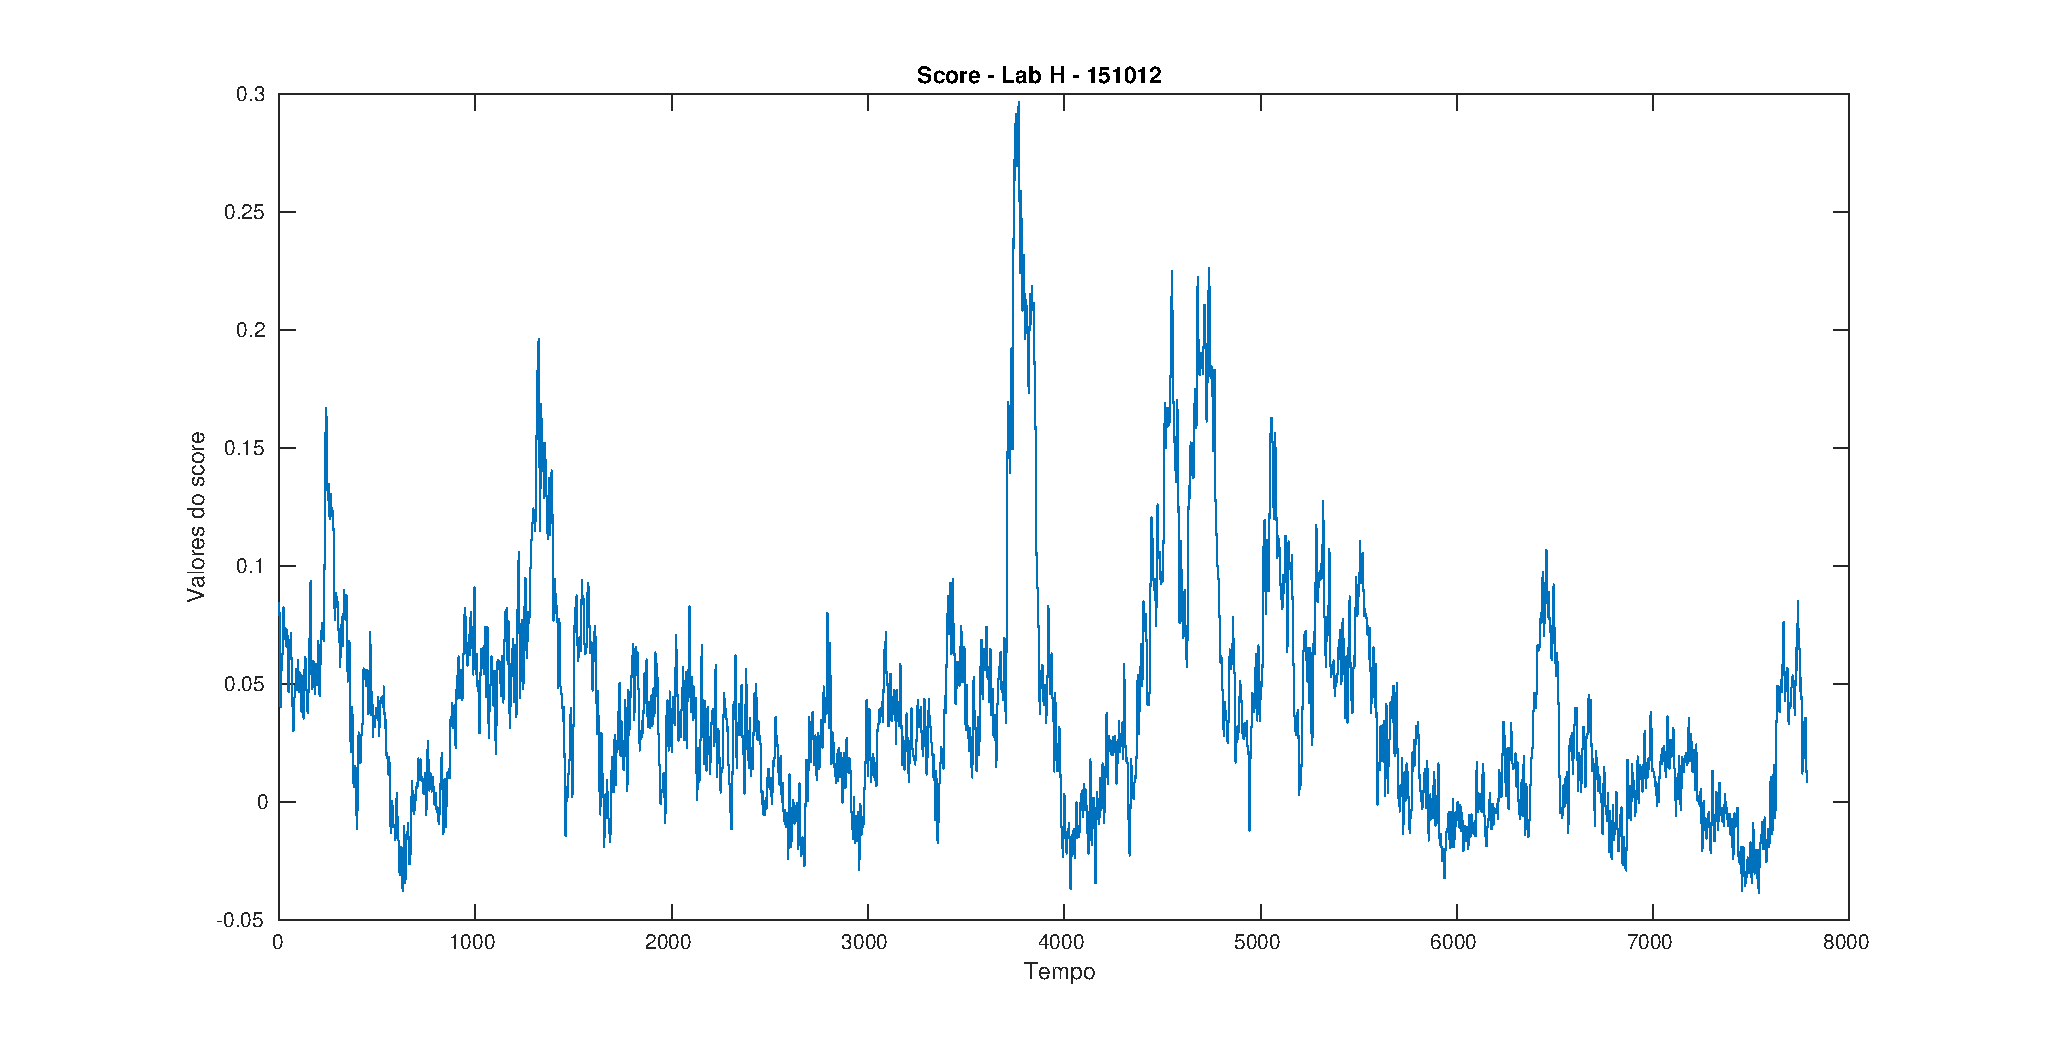
\includegraphics[width=0.5\textwidth]{figuras/GW151012_LabH.eps}}
     \subfigure[Score gerado para o laboratório L]{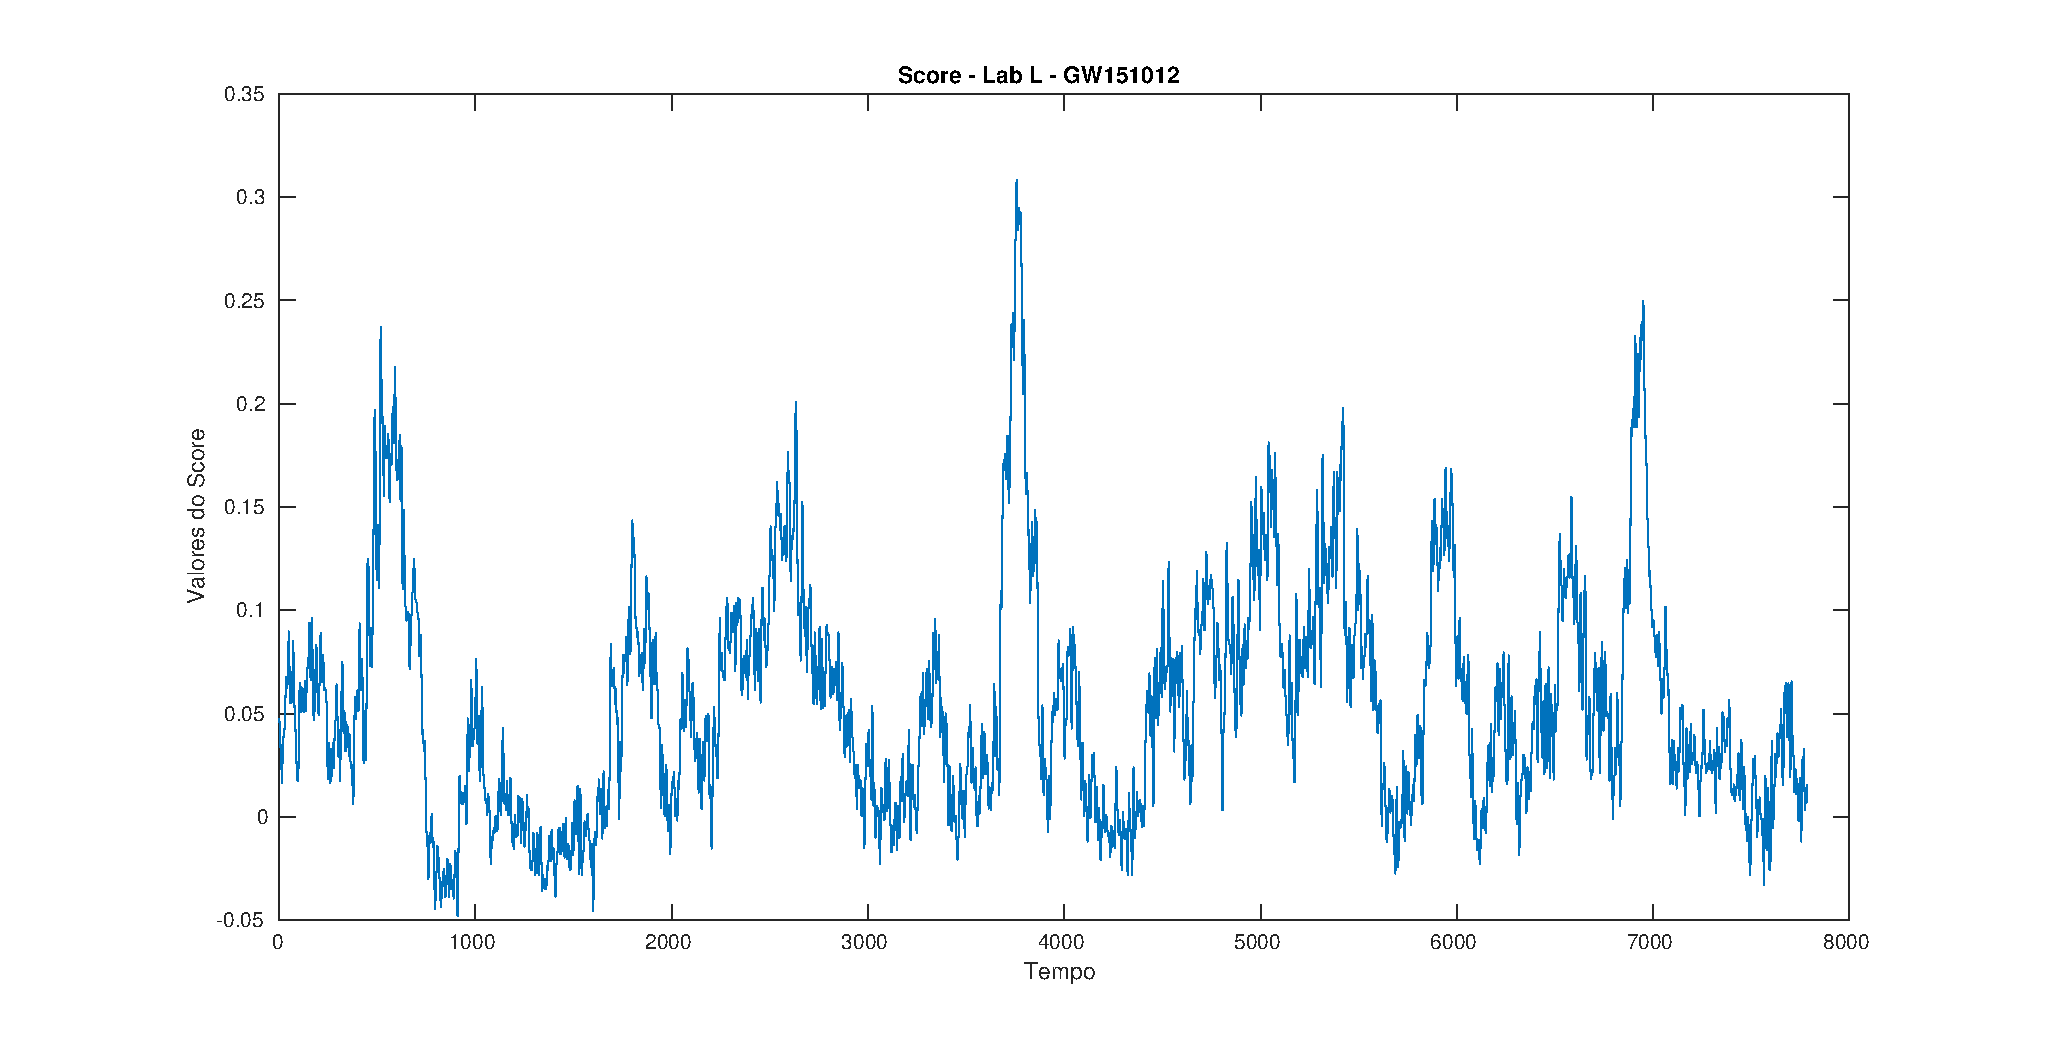
\includegraphics[width=0.5\textwidth]{figuras/GW151012_LabL.eps}}
     \subfigure[Coincidência entre os dois scores]{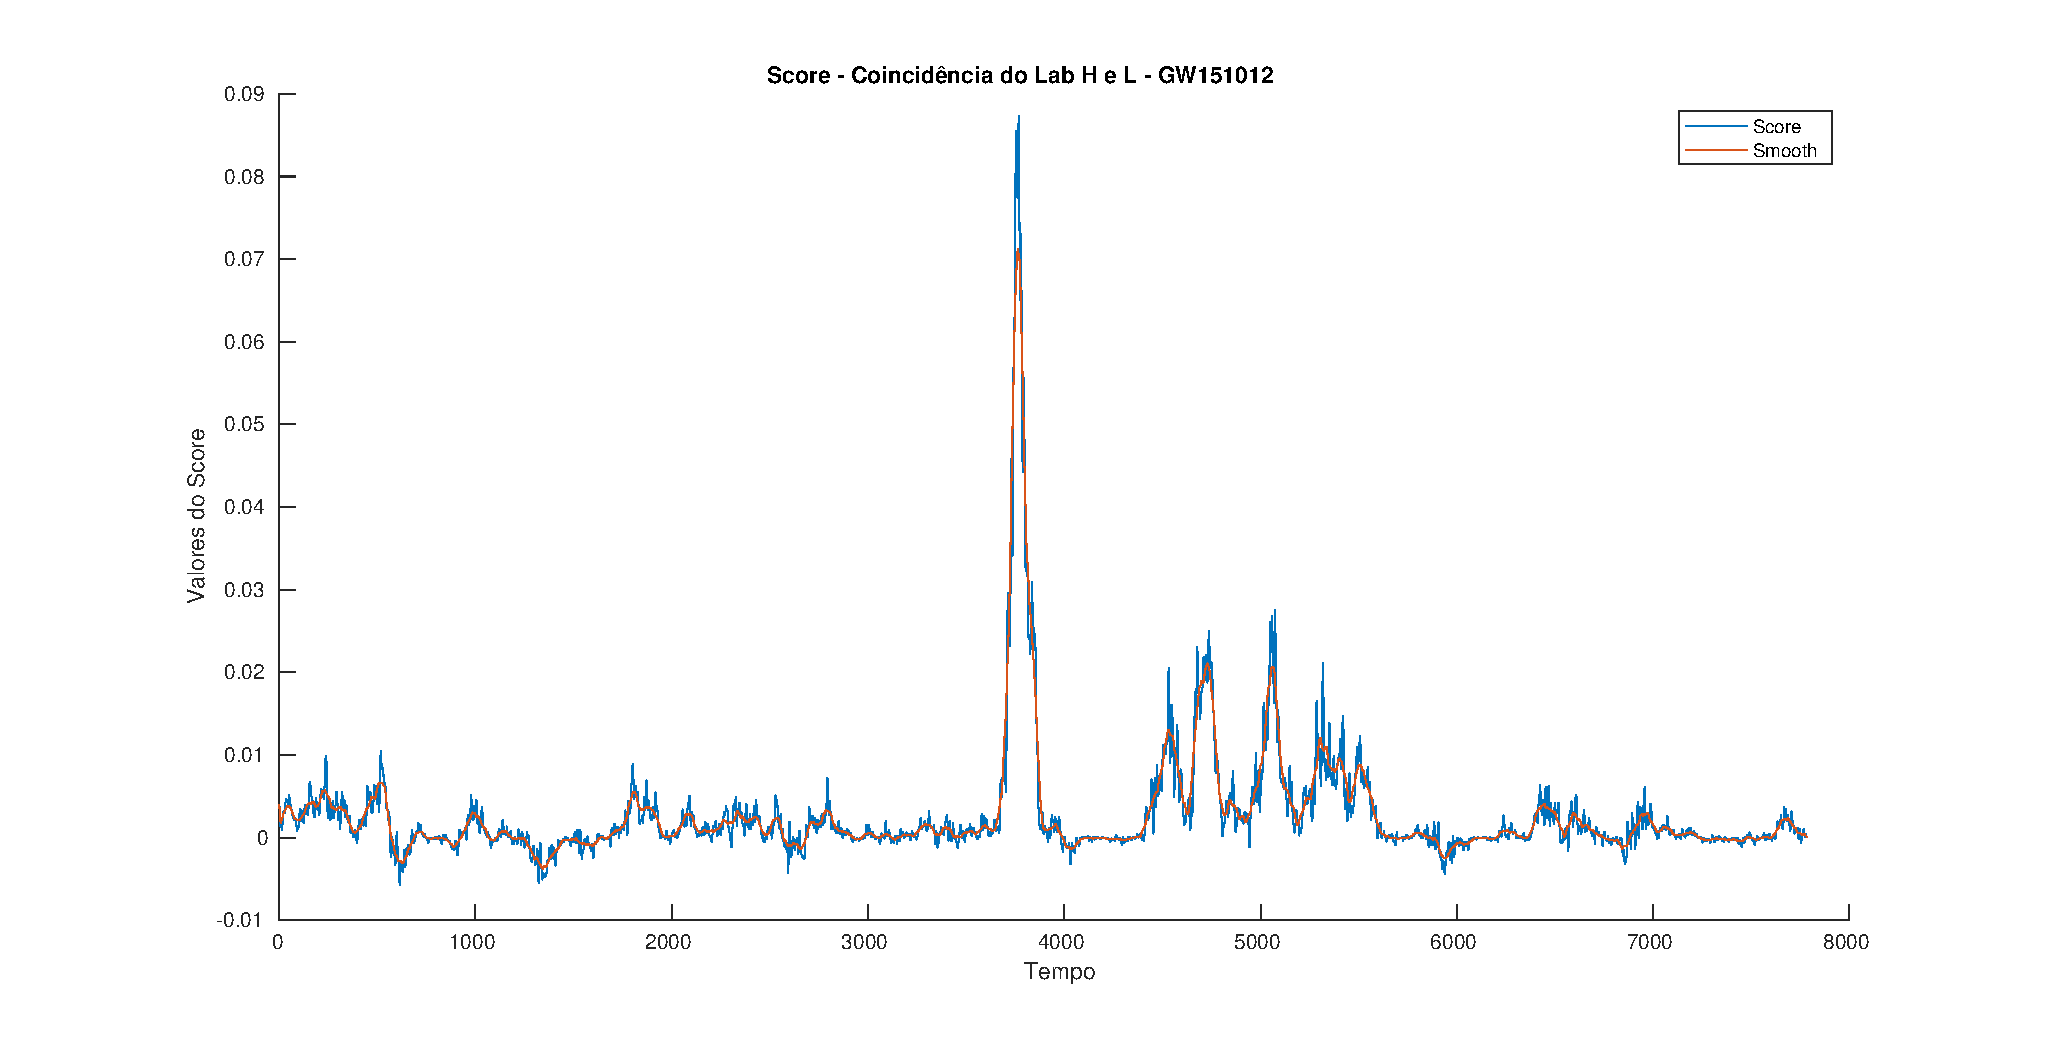
\includegraphics[width=1.0\textwidth]{figuras/GW151012_LabHL.eps}}
     \caption{Score da onda gravitacional GW151012}
 \end{figure*}
	
% 	\imprimiranexos
% 		% Adicione aqui os anexos do seu trabalho
% 		\input{elementos-pos-textuais/anexos/exemplo-de-anexo}
	\imprimirindice

\end{document}